\documentclass[a5paper]{article}

\usepackage{amsmath, amssymb}
\usepackage{multicol}
\setlength{\columnsep}{1cm}
\usepackage[margin=0.75in]{geometry}
\usepackage{graphicx}
\graphicspath{ {../../../Images/ENEX12002/} }
\usepackage[breaklinks, hidelinks]{hyperref}
\usepackage{siunitx}
\usepackage{tikz}
\usetikzlibrary{patterns, positioning, arrows.meta}
\usepackage[american]{circuitikz}
\usepackage{pgfplots}
\pgfplotsset{compat=newest}
\usepgfplotslibrary{external}
\usepackage{stix}
\usepackage{ragged2e}
\usepackage{enumitem}
\usepackage{polynom}

\newcommand{\minus}{\scalebox{0.5}[1.0]{$-$}}
\newcommand{\sech}{\mathrm{sech}}
\newcommand{\csch}{\mathrm{csch}}
\setcounter{secnumdepth}{4}
\renewcommand\paragraph{\@startsection{paragraph}{4}{\z@}%
% display heading, like subsubsection
                                     {-3.25ex\@plus -1ex \@minus -.2ex}%
                                     {1.5ex \@plus .2ex}%
                                     {\normalfont\normalsize\bfseries}}
\sisetup{
	round-mode = places,
	round-precision = 2,
}

\date{2\textsuperscript{nd} of July 2026}

\begin{document}
	\begin{titlepage}
		\centering
		{\Huge \textsc{ENEX12002}\par}
		\vspace{1cm}
		{\Large \textsc{Lecture Notes}\par}
		\vspace{2.5cm}
		\vfill
		Authored by\par
		Lachlan J. W. Wyer
		\vfill
		\makeatletter
		{\large Document Start Date: \@date \par}
		\makeatother
		{\large Latest Update: \today\par}
	\end{titlepage}
	\tableofcontents
	\pagebreak

	\section{Analog Circuits}
	\subsection{Characteristic Curves:}
	A characteristic curve is a type of linear plot that demonstates a relationship between two variable properties of a device. Most electronic devices CC refers too a plot of current as a function of coltage. Mostly known as an I-V curve.
	\begin{center}
	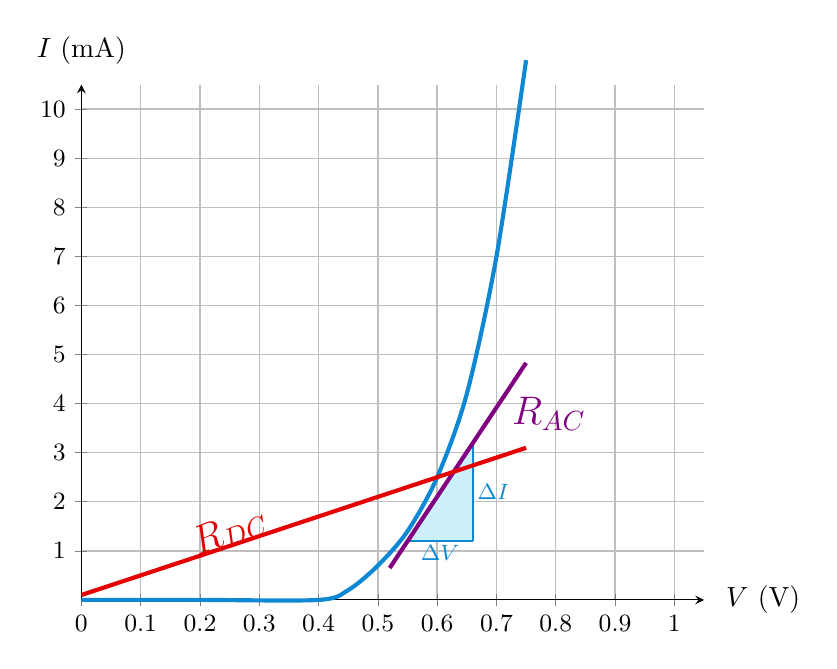
\begin{tikzpicture}
	    \begin{axis}[
		scale=0.75,
		width=\textwidth,
		height=0.85\textwidth,
		xmin=0, xmax=1.05,
		ymin=0, ymax=10.5,
		xtick={0, 0.1, 0.2, 0.3, 0.4, 0.5, 0.6, 0.7, 0.8, 0.9, 1.0},
		ytick={1, 2, 3, 4, 5, 6, 7, 8, 9, 10},
		xlabel={$V \text{ (V)}$},
		ylabel={$I \text{ (mA)}$},
		axis lines=left,
		grid=both,
		major grid style={line width=0.5pt,draw=gray!50},
		minor grid style={line width=0.2pt,draw=gray!20},
		every axis x label/.style={at={(ticklabel* cs:1.02)},anchor=west, font=\normalsize},
		every axis y label/.style={at={(ticklabel* cs:1.02)},anchor=south, font=\normalsize},
		tick label style={font=\small},
		enlargelimits=false,
		clip=false
	    ]
	    
	    % Diode curve (Approximation of the non-linear I-V characteristic)
	    \addplot [color=cyan!70!blue, line width=1.5pt, smooth] coordinates {
		(0,0) (0.2,0) (0.4,0) (0.45, 0.2) (0.5, 0.7) (0.55, 1.4) (0.6, 2.5) (0.65, 4.2) (0.7, 7.0) (0.75, 11)
	    };
	    
	    % Delta V, Delta I filled triangle area
	    \fill [cyan!20] (0.55, 1.2) -- (0.66, 1.2) -- (0.66, 3.2) -- cycle;
	    
	    % Triangle outline and Delta annotations
	    \draw [color=cyan!70!blue, thick] (0.55, 1.2) -- (0.66, 1.2) node[midway, below, font=\footnotesize, yshift=2pt] {$\Delta V$};
	    \draw [color=cyan!70!blue, thick] (0.66, 1.2) -- (0.66, 3.2) node[midway, right, font=\footnotesize, xshift=-2pt] {$\Delta I$};
	    
	    % R_AC line (Purple Tangent Line representing dynamic resistance)
	    \draw [color=violet, line width=1.5pt] (0.52, 0.65) -- (0.75, 4.83);
	    \node [color=violet, font=\Large\bfseries, right] at (0.71, 3.8) {$R_{AC}$};
	    
	    % R_DC line (Red Secant Line representing static resistance)
	    \draw [color=red!90!black, line width=1.5pt] (0, 0.1) -- (0.75, 3.1);
	    \node [color=red!90!black, font=\Large\bfseries, rotate=22] at (0.25, 1.4) {$R_{DC}$};
	    
	    \end{axis}
	\end{tikzpicture}
	\end{center}
	\subsection{Analog vs Digital Signals:}
	Signalling within a circuit is generally classified as either continuous or discrete. Continuous (Analog signalling) varies after a range of values within limits. Discrete (Digital signals) change between two discreet voltage levels.
	\begin{center}
	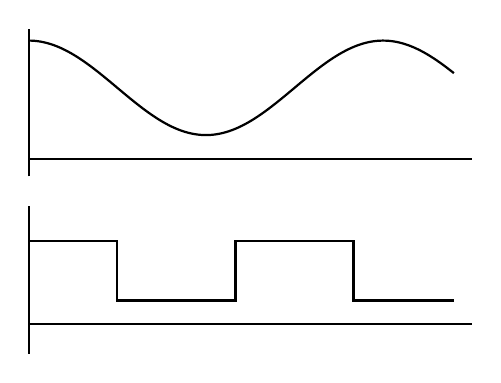
\begin{tikzpicture}[scale=0.75, transform shape]

	    % --- Top Plot (Analog / Smooth Waveform) ---
	    % Y and X Axes
	    \draw[thick] (0, 2.5) -- (0, 5.0);
	    \draw[thick] (0, 2.8) -- (7.5, 2.8);
	    
	    % Smooth curve (Modeled as a cosine wave with a DC offset)
	    \draw[thick] plot[domain=0:7.2, samples=150] (\x, {4.0 + 0.8 * cos(60*\x)});

	    % --- Bottom Plot (Digital / Square Waveform) ---
	    % Y and X Axes
	    \draw[thick] (0, -0.5) -- (0, 2.0);
	    \draw[thick] (0, 0) -- (7.5, 0); 
	    
	    % Square wave path (with DC offset)
	    \draw[thick] (0, 1.4) -- (1.5, 1.4) 
			 -- (1.5, 0.4) -- (3.5, 0.4) 
			 -- (3.5, 1.4) -- (5.5, 1.4) 
			 -- (5.5, 0.4) -- (7.2, 0.4);

	\end{tikzpicture}
	\end{center}
	\subsection{Analog \& Digital Circuits:}
	Analog circuits are used in situations implementing linear functions, wave shaping and transformation between current and voltage. Digital circuit however ase used to process data rapidly and in calculations. Most systems utilize a mix of both systems (e.g AV systems).
	\subsection{Sampling:}
	When converting between signal types sampling must take place. Sampling is the approximation of analog's original waveform into time slices. The disadvantage of sampling is that is loses some precision, however the advantages of a digital system out weight this. The physical process of sampling is called quantizing. This produces numbers that can be processed by digital systems.
	\begin{center}
		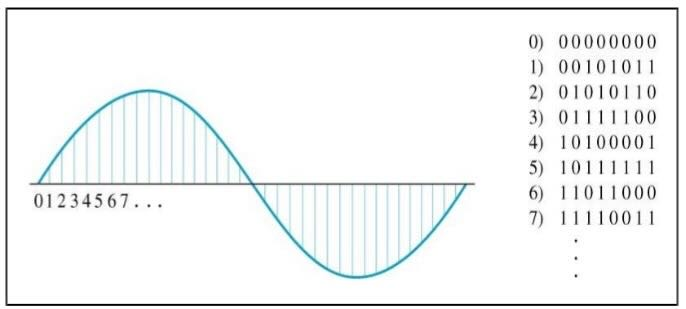
\includegraphics[scale=0.5]{quantizing-example.png}
	\end{center}
	\subsection{Vectors:}
	A vector is a line that contains both direction and magnitude. An AC circuits sinusodial waveform can be generated by plotting the project of a rotating vector in circular motion.
	\subsection{Frequency and Period:}
	The frequency of a periodic wave is the number of cycles that occur every second. The SI unit for this is Hz. The period is how long it takes a waveform to complete one cycle.
	$$f=\frac{1}{T}$$
	$$T=\frac{1}{f}$$
	\subsection{Instantaneous Values:}
	$$v(t)=V_{p}\sin{(\omega t\pm\phi)}$$
	The instantaneous values are always against time ($t$).
	\begin{center}
	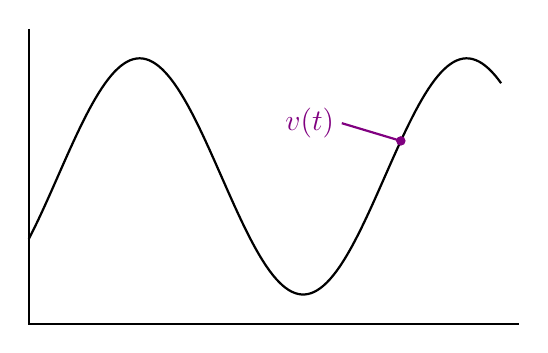
\begin{tikzpicture}[scale=0.75, transform shape]

	    % --- Axes ---
	    % Y and X Axes (drawn with a slight extension past the origin for standard styling)
	    \draw[thick] (0.2, 5.0) -- (0.2, 0) -- (8.5, 0);

	    % --- Waveform ---
	    % Modeled as a smooth sine wave with a DC offset to match the sketch
	    \draw[thick] plot[domain=0.2:8.2, samples=150] (\x, {2.5 + 2*sin(65*\x - 45)});

	    % --- Annotation ---
	    % Coordinate placed on the rising edge of the second cycle
	    \coordinate (VT) at (6.5, {2.5 + 2*sin(65*6.5 - 45)});
	    
	    % Draw the marker point
	    \filldraw[violet] (VT) circle (2pt);
	    
	    % Draw the label line and text
	    \draw[violet, thick] (VT) -- ++(-1.0, 0.3) node[left, font=\Large\bfseries] {$v(t)$};

	\end{tikzpicture}
	\end{center}
	\subsection{Waveform Values:}
	The amplitude is the maximum distance of the values from the line of equilibrium. The average value of a sine wave is the found in $\lvert v(t) \rvert$, then averaging the curve.
	$$V_{ave}=\frac{2V_{p}}{\pi}\approx 0.637V_{p}$$
	\subsection{RMS Values:}
	In order to compare AC and DC currents and voltages, AC is converted into its DC equivalent DC heating value. RMS current and voltage are their peak values.
	\begin{align*}
		V_{RMS}=&\frac{V_{p}}{\sqrt{2}}\\
		\approx & 0.707V_{p}\\\\
		I_{RMS}=&\frac{I_{p}}{\sqrt{2}}\\
		\approx & 0.707I_{p}
	\end{align*}
	\subsection{Domain Signals:}
	Time domain is the funcation against time. An example is a oscciliscope which shows values over a period of time. The frequency domain - A sine-wave against time can be represented against its frequency. This representations shows the waveforms amplitude and frequency but not it's phase angle.
	\begin{center}
		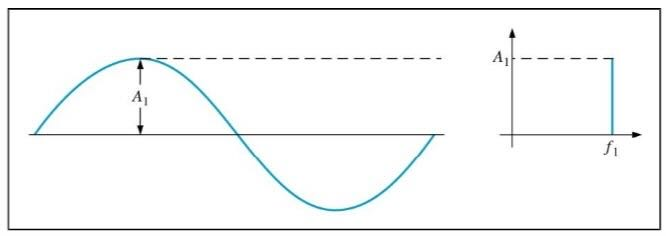
\includegraphics[scale=0.5]{domain-signals.png}
	\end{center}
	\subsection{Transducers:}
	These are a device that converts a physical quantity (e.g pressure, position or temp) from one form to another. Their outupts are quite small and require amplification. Passice transducers require external power to functions, this is called excitation. Active transducers are self-generating that convert a portion being measured into electrical signal.
	\subsection{Amplification:}
	Amps are designde to amplify either voltage or power. Linear amplifiers produce a magnified replica of the inputted signal, producing a useful output.
	$$A_{v}=\frac{V_{out}}{V_{in}}$$
	\subsection{Transfer Curves:}
	All amplifiers, when ideal, produce a linear transfer curves. Beyond this limit they no longer act idealy, this is called saturation.
	\subsection{Power Gain:}
	$$A_{p}=\frac{P_{out}}{P_{in}}=\frac{V_{out}I_{out}}{V_{in}I_{in}}$$
	\subsection{dB Power Ratios:}
	The decibal of a power ratio is:
	\begin{align*}
		A_{p}=&10\log_{10}{(\frac{P_{1}}{P_{2}})}\\
		=&10\log_{10}{(A_{p})}
	\end{align*}
	\subsection{dB Voltage Ratio:}
	\begin{align*}
		A_{v}=&20\log_{10}{(\frac{V_{1}}{V_{2}})}\\
		=&20\log_{10}{(A_{v})}
	\end{align*}

	\section{Basic Circuit Theory}
	\subsection{Electrical Charge:}
	Electrical effects are attributed to the seperation of charges and their movements. Electrical forces are that opposites attract and similar repels. A charge is considered continuous if $q=1.6022E\minus19e^{-}$.
	\subsection{Voltage and Current:}
	Rather than working purely in charge, it is easier to work with it in voltage and current.
	$$V=\frac{dw}{dq}$$
	$$I=\frac{dq}{dt}$$
	\subsection{Ideal Basic Circuits:}
	These are made up of 5 main points:
	\begin{enumerate}
		\item Two Terminals
		\item Can be described mathmatically in terms of voltage and current
		\item Cannot be subdivided into further elements
		\item Utilizes the passive sign convention
	\end{enumerate}
	\begin{center}
	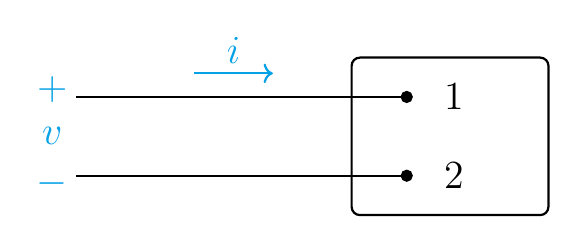
\begin{tikzpicture}[scale=1, transform shape]

	    % --- Wires ---
	    % Wires extending from the left into the network box
	    \draw[thick] (0, 1.5) -- (4.2, 1.5);
	    \draw[thick] (0, 0.5) -- (4.2, 0.5);

	    % --- Network Box ---
	    % Drawn as a simple rectangle encompassing the terminals
	    \draw[thick, rounded corners=3pt] (3.5, 0) rectangle (6, 2);

	    % --- Terminals ---
	    % Top terminal (Node 1)
	    \filldraw (4.2, 1.5) circle (2pt);
	    \node[font=\Large] at (4.8, 1.5) {1};
	    
	    % Bottom terminal (Node 2)
	    \filldraw (4.2, 0.5) circle (2pt);
	    \node[font=\Large] at (4.8, 0.5) {2};

	    % --- Voltage Annotations (Blue) ---
	    \node[cyan!90!blue, font=\Large\bfseries] at (-0.3, 1.6) {$+$};
	    \node[cyan!90!blue, font=\Large\bfseries] at (-0.3, 1.0) {$v$};
	    \node[cyan!90!blue, font=\Large\bfseries] at (-0.3, 0.4) {$-$};

	    % --- Current Annotation (Blue) ---
	    % Arrow indicating current flow direction on the top wire
	    \draw[cyan!90!blue, thick, ->] (1.5, 1.8) -- (2.5, 1.8) node[midway, above, font=\Large\bfseries] {$i$};

	\end{tikzpicture}
	\end{center}
	\subsection{Power and Energy:}
	The useful output of a system is often non-electrical. Practical applications also have limitations in the amount of power it can handle.
	$$p=\frac{dw}{dt}=(\frac{dw}{dq})(\frac{dq}{dt})=VI$$
	The polarity describes where current flows in the relationship to voltage. If $p>0$, power is being delivered to the circuit inside the box. For instance a motor.
	\begin{center}
	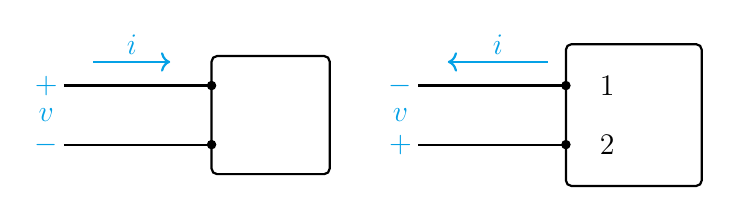
\begin{tikzpicture}[scale=0.75, transform shape]

	    % Define color for annotations to match sketch
	    \colorlet{anncolor}{cyan!90!blue}

	    % ==========================================
	    % LEFT DIAGRAM 
	    % ==========================================
	    
	    % Wires
	    \draw[thick] (0, 1.5) -- (2.5, 1.5);
	    \draw[thick] (0, 0.5) -- (2.5, 0.5);

	    % Network Box
	    \draw[thick, rounded corners=2pt] (2.5, 0) rectangle (4.5, 2);

	    % Terminals
	    \filldraw (2.5, 1.5) circle (2pt);
	    \filldraw (2.5, 0.5) circle (2pt);

	    % Voltage Annotations
	    \node[anncolor, font=\Large\bfseries] at (-0.3, 1.5) {$+$};
	    \node[anncolor, font=\Large\bfseries] at (-0.3, 1.0) {$v$};
	    \node[anncolor, font=\Large\bfseries] at (-0.3, 0.5) {$-$};

	    % Current Annotation (Arrow pointing Right)
	    \draw[anncolor, thick, ->] (0.5, 1.9) -- (1.8, 1.9) node[midway, above, font=\Large\bfseries] {$i$};

	    % ==========================================
	    % RIGHT DIAGRAM 
	    % ==========================================
	    
	    % Shift entire right diagram by 6 units to place it side-by-side
	    \begin{scope}[xshift=6cm]
		% Wires
		\draw[thick] (0, 1.5) -- (2.5, 1.5);
		\draw[thick] (0, 0.5) -- (2.5, 0.5);

		% Network Box 
		\draw[thick, rounded corners=2pt] (2.5, -0.2) rectangle (4.8, 2.2);

		% Terminals and Labels
		\filldraw (2.5, 1.5) circle (2pt);
		\node[font=\Large] at (3.2, 1.5) {1};
		
		\filldraw (2.5, 0.5) circle (2pt);
		\node[font=\Large] at (3.2, 0.5) {2};

		% Voltage Annotations (Reversed polarity from left diagram)
		\node[anncolor, font=\Large\bfseries] at (-0.3, 1.5) {$-$};
		\node[anncolor, font=\Large\bfseries] at (-0.3, 1.0) {$v$};
		\node[anncolor, font=\Large\bfseries] at (-0.3, 0.5) {$+$};

		% Current Annotation (Arrow pointing Left)
		\draw[anncolor, thick, <-] (0.5, 1.9) -- (2.2, 1.9) node[midway, above, font=\Large\bfseries] {$i$};
	    \end{scope}
	\end{tikzpicture}
	\end{center}
	Else if $p<0$, power is being extracted from a circuit. For example a battery.
	\begin{center}
	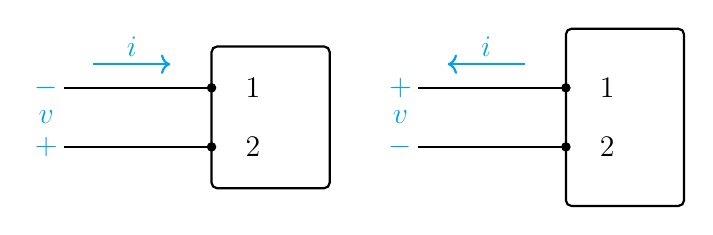
\begin{tikzpicture}[scale=0.75, transform shape]

	    % Define color for annotations to match sketch
	    \colorlet{anncolor}{cyan!90!blue}

	    % ==========================================
	    % LEFT DIAGRAM 
	    % ==========================================
	    
	    % Wires
	    \draw[thick] (0, 1.5) -- (2.5, 1.5);
	    \draw[thick] (0, 0.5) -- (2.5, 0.5);

	    % Network Box
	    \draw[thick, rounded corners=2pt] (2.5, -0.2) rectangle (4.5, 2.2);

	    % Terminals and Labels
	    \filldraw (2.5, 1.5) circle (2pt);
	    \node[font=\Large] at (3.2, 1.5) {1};
	    
	    \filldraw (2.5, 0.5) circle (2pt);
	    \node[font=\Large] at (3.2, 0.5) {2};

	    % Voltage Annotations (- on top, + on bottom)
	    \node[anncolor, font=\Large\bfseries] at (-0.3, 1.5) {$-$};
	    \node[anncolor, font=\Large\bfseries] at (-0.3, 1.0) {$v$};
	    \node[anncolor, font=\Large\bfseries] at (-0.3, 0.5) {$+$};

	    % Current Annotation (Arrow pointing Right)
	    \draw[anncolor, thick, ->] (0.5, 1.9) -- (1.8, 1.9) node[midway, above, font=\Large\bfseries] {$i$};

	    % ==========================================
	    % RIGHT DIAGRAM 
	    % ==========================================
	    
	    % Shift entire right diagram by 6 units to place it side-by-side
	    \begin{scope}[xshift=6cm]
		% Wires
		\draw[thick] (0, 1.5) -- (2.5, 1.5);
		\draw[thick] (0, 0.5) -- (2.5, 0.5);

		% Network Box 
		\draw[thick, rounded corners=2pt] (2.5, -0.5) rectangle (4.5, 2.5);

		% Terminals and Labels
		\filldraw (2.5, 1.5) circle (2pt);
		\node[font=\Large] at (3.2, 1.5) {1};
		
		\filldraw (2.5, 0.5) circle (2pt);
		\node[font=\Large] at (3.2, 0.5) {2};

		% Voltage Annotations (+ on top, - on bottom)
		\node[anncolor, font=\Large\bfseries] at (-0.3, 1.5) {$+$};
		\node[anncolor, font=\Large\bfseries] at (-0.3, 1.0) {$v$};
		\node[anncolor, font=\Large\bfseries] at (-0.3, 0.5) {$-$};

		% Current Annotation (Arrow pointing Left)
		\draw[anncolor, thick, <-] (0.5, 1.9) -- (1.8, 1.9) node[midway, above, font=\Large\bfseries] {$i$};
	    \end{scope}

	\end{tikzpicture}
	\end{center}
	Elements that make up a basic circui include:
	\begin{itemize}
		\item Voltage source/s
		\item Current source/s
		\item Passive Circuit elements, As they do not produce electricity
			\begin{itemize}
				\item Resistors
				\item Inductors
				\item Capacitors
			\end{itemize}
	\end{itemize}
	\subsection{Voltage and Current Sources:}
	An electrical source that can convert between electrical and non-electrical energy. An ideal voltage source provides a consistant voltage regardless of current. This is similar for current sources. In real-world applications, ideal power sources do not exist.
	\subsubsection{Source Types}
	\begin{center}
	\begin{circuitikz}[scale=1.3, transform shape, line width=0.8pt]

	    % Define a custom purple color to match the handwritten annotations
	    \definecolor{annpurple}{RGB}{95, 40, 130}

	    % ==========================================
	    % TOP ROW: INDEPENDENT SOURCES
	    % ==========================================
	    
	    % Independent Voltage Source (+ on top, - on bottom)
	    % Drawing from bottom to top puts the '+' at the top coordinate.
	    % 'l=' places the label on the left side of the path.
	    \draw (0, 0) to[V, invert, l=$V_s$] (0, 2.5);
	    
	    % Independent Current Source (arrow pointing up)
	    \draw (3, 0) to[I, l=$i_s$] (3, 2.5);
	    
	    % Text Annotation
	    \node[annpurple, font=\Large\bfseries, align=left, right] at (4.5, 1.25) {Independent\\Sources};

	    % ==========================================
	    % BOTTOM ROW: DEPENDENT SOURCES
	    % ==========================================
	    
	    % Dependent Voltage Source (+ on top, - on bottom)
	    % 'cV' denotes a controlled (dependent) voltage source.
	    \draw (0, -3.5) to[cV, invert, l=$V_s$] (0, -1);
	    
	    % Dependent Current Source (arrow pointing up)
	    % 'cI' denotes a controlled (dependent) current source.
	    \draw (3, -3.5) to[cI, l=$i_s$] (3, -1);
	    
	    % Text Annotation
	    \node[annpurple, font=\Large\bfseries, align=left, right] at (4.5, -2.25) {Dependent\\Sources};
	\end{circuitikz}
	\end{center}
	\subsection{Kirchoffs Laws:}
	A circuit is said to be solved once a voltage and current is found across every circuit element.
	$$\text{KCL}\;\Rightarrow\;\sum I_{out}=\sum I_{in}$$
	$$\text{KVL}\;\Rightarrow\;\sum V_{loop}=0$$
	To apply these laws, polarity must be applied throughout the circuit.
	\subsection{Resistance:}
	Resistors resist the flow of current within a circuit. Conductance is also the inverse of resistance, $G=\frac{1}{R}$.
	\begin{center}
	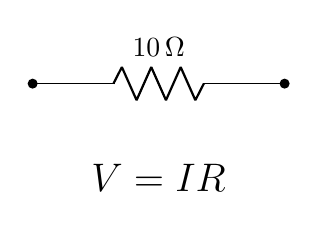
\begin{tikzpicture}[scale=0.8]
		
		% Draw the resistor with 10 ohm label and filled nodes at ends
		\draw (0,0) to[R, l=\SI{10}{\ohm}, *-*] (4,0);
		
		% Add the V = IR equation below the resistor
		\node at (2, -1.5) {\Large $V = IR$};
		
	\end{tikzpicture}
	\end{center}
	\subsubsection{Series}
	$$R_{eq}=\sum^{k}_{n=1}\;R_{n}$$
	\begin{center}
	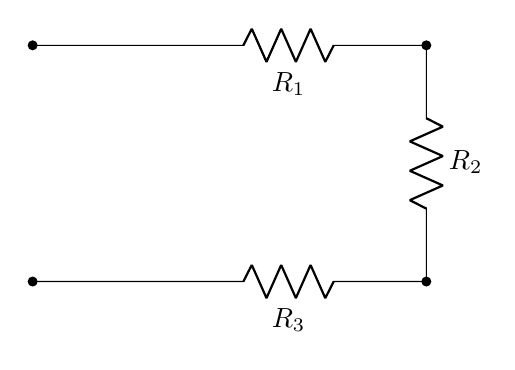
\begin{tikzpicture}
		\draw (0,3) to[short, *-] (1.5,3) 
			    to[R, l_=$R_1$, -*] (5,3)
			    to[R, l=$R_2$, -*] (5,0)
			    to[R, l=$R_3$, -] (1.5,0)
			    to[short, -*] (0,0);
	\end{tikzpicture}
	\end{center}
	\subsubsection{Parllel}
	$$R_{eq}=\frac{1}{\sum^{k}{n=1}\frac{1}{R_{n}}}$$
	\begin{center}
	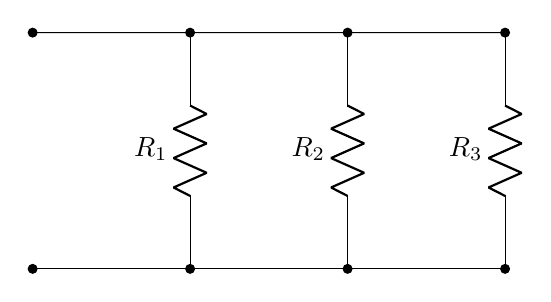
\begin{tikzpicture}
		% Top and bottom terminals connecting to the first branch
		\draw (0,3) to[short, *-*] (2,3);
		\draw (0,0) to[short, *-*] (2,0);
		
		% First resistor branch (R1)
		\draw (2,3) to[R, l_=$R_1$] (2,0);
		
		% Connecting to second branch
		\draw (2,3) to[short, -*] (4,3);
		\draw (2,0) to[short, -*] (4,0);
		
		% Second resistor branch (R2)
		\draw (4,3) to[R, l_=$R_2$] (4,0);
		
		% Connecting to third branch
		\draw (4,3) to[short, -*] (6,3);
		\draw (4,0) to[short, -*] (6,0);
		
		% Third resistor branch (R3)
		\draw (6,3) to[R, l_=$R_3$] (6,0);
	\end{tikzpicture}
	\end{center}
	\subsection{Voltage Division:}
	$$V_{j}=iR_{j}=\frac{R_{j}}{R_{eq}}V$$
	\begin{center}
	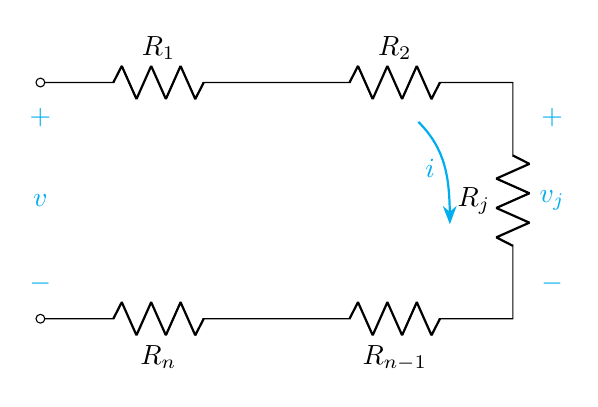
\begin{tikzpicture}
		% Main circuit branches
		\draw (0,3) to[R, l=$R_1$, o-] (3,3)
			    to[R, l=$R_2$] (6,3)
			    to[R, l_=$R_j$] (6,0)
			    to[R, l=$R_{n-1}$] (3,0)
			    to[R, l=$R_n$, -o] (0,0);
		
		% Input voltage v (cyan to match the sketch's blue ink)
		\draw[cyan] (0,3) to[open, v=$v$] (0,0);
		
		% Voltage v_j across R_j
		\draw[cyan] (6.5,3) to[open, v^=$v_j$] (6.5,0);
		
		% Curved current arrow i
		\draw[-{Stealth}, cyan, thick] (4.8, 2.5) to[out=-45, in=90] node[midway, left] {$i$} (5.2, 1.2);
	\end{tikzpicture}
	\end{center}
	\subsection{Current Division:}
	$$i_{j}=\frac{V}{R_{j}}=\frac{R_{eq}}{R_{j}}i$$
	\begin{center}
	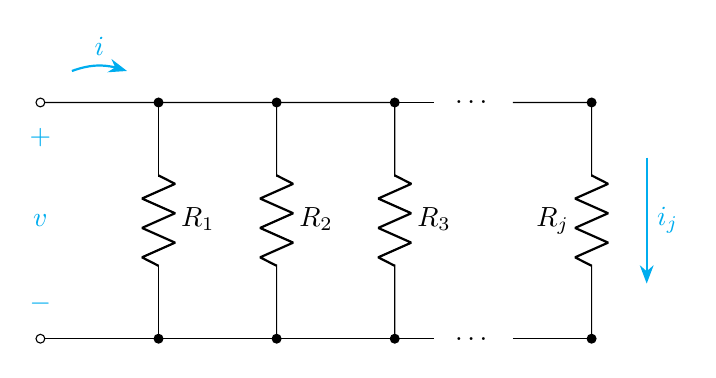
\begin{tikzpicture}
		% Terminals and top/bottom rails to first resistor
		\draw (0,3) to[short, o-*] (1.5,3);
		\draw (0,0) to[short, o-*] (1.5,0);
		
		% Input voltage v
		\draw[cyan] (0,3) to[open, v=$v$] (0,0);
		
		% Input current i
		\draw[-{Stealth}, cyan, thick] (0.4, 3.4) to[out=20, in=160] node[midway, above] {$i$} (1.1, 3.4);
		
		% First parallel branch (R1)
		\draw (1.5,3) to[R, l=$R_1$] (1.5,0);
		
		% Second parallel branch (R2)
		\draw (1.5,3) to[short, -*] (3,3);
		\draw (1.5,0) to[short, -*] (3,0);
		\draw (3,3) to[R, l=$R_2$] (3,0);
		
		% Third parallel branch (R3)
		\draw (3,3) to[short, -*] (4.5,3);
		\draw (3,0) to[short, -*] (4.5,0);
		\draw (4.5,3) to[R, l=$R_3$] (4.5,0);
		
		% Ellipses for continuation
		\draw (4.5,3) -- (5,3);
		\draw (4.5,0) -- (5,0);
		\node at (5.5, 3) {$\dots$};
		\node at (5.5, 0) {$\dots$};
		\draw (6,3) to[short, -*] (7,3);
		\draw (6,0) to[short, -*] (7,0);
		
		% Branch j (R_j)
		\draw (7,3) to[R, l_=$R_j$] (7,0);
		
		% Current i_j across R_j
		\draw[-{Stealth}, cyan, thick] (7.7, 2.3) -- node[right] {$i_j$} (7.7, 0.7);
	\end{tikzpicture}
	\end{center}
	\subsection{Source Transformations:}
	Current and voltage sources can be interchanged. This is because equivalent sources produce the same electrical effects, regardless of load.
	\subsubsection{Th\'evenin Equivalent}
	A way to simplify a circuit that focuses on the behaviour at the terminals.
	$$V_{TH}=V_{O/C}=V_{ab}$$
	$$R_{TH}=\frac{V_{TH}}{I_{SC}}$$
	\begin{center}
	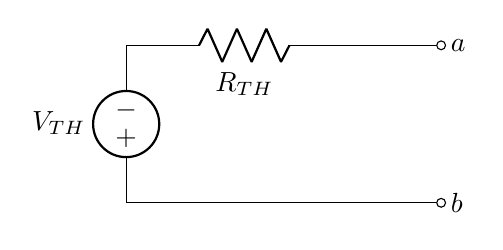
\begin{tikzpicture}
		% Top Circuit
		\draw (0,0) to[V, l=$V_{TH}$] (0,2)
				to[R, l_=$R_{TH}$] (3,2)
				to[short, -o] (4,2) node[right] {$a$};
		\draw (0,0) to[short, -o] (4,0) node[right] {$b$};
	\end{tikzpicture}
	\end{center}
	\subsubsection{Norton Equivalent}
	$$I_{N}=I_{S/C}$$
	$$R_{N}=R_{TH}$$
	\begin{center}
	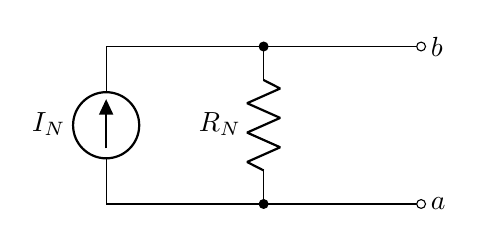
\begin{tikzpicture}
		% Bottom Circuit
		\draw (0,-4) to[I, l=$I_N$] (0,-2)
			     to[short, -*] (2,-2)
			     to[short, -o] (4,-2) node[right] {$b$};
			     
		\draw (2,-2) to[R, l_=$R_{N}$] (2,-4);
		
		\draw (0,-4) to[short, -*] (2,-4)
			     to[short, -o] (4,-4) node[right] {$a$};
	\end{tikzpicture}
	\end{center}
	\subsection{Maximum Power:}
	To find a circuits maximum power, replace its resistive network within its Th\'ev\-enin equivalent.
	\begin{center}
	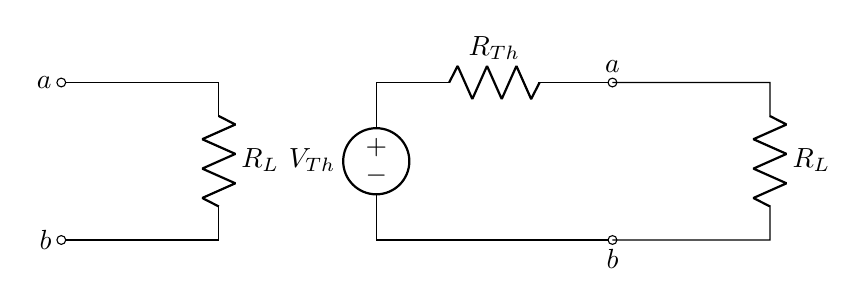
\begin{tikzpicture}[scale=1]
		% Left Circuit
		\draw (0,2) node[left] {$a$} to[short, o-] (2,2)
			    to[R, l=$R_L$] (2,0)
			    to[short, -o] (0,0) node[left] {$b$};
		
		% Right Circuit - Thevenin Equivalent
		\draw (4,0) to[V, invert, l=$V_{Th}$] (4,2)
			    to[R, l=$R_{Th}$, -o] (7,2) node[above] {$a$};
		
		\draw (4,0) to[short, -o] (7,0) node[below] {$b$};
		
		% Right Circuit - Load attached to terminals
		\draw (7,2) to[short] (9,2)
			    to[R, l=$R_L$] (9,0)
			    to[short] (7,0);
	\end{tikzpicture}
	\end{center}
	Power delivery to $R_{L}$:
	$$p=I^{2}R_{L}=(\frac{V_{TH}}{R_{TH}+R_{L}})^{2}R_{L}$$
	Max power is when $R_{L}=R_{TH}$:
	$$p_{max}=\frac{V_{TH}^{2}R_{L}}{(2R_{L})^{2}}=\frac{V_{TH}^{2}}{4R_{L}}$$
	\subsection{Superposition Principle:}
	A linear system obeys this principle. Which is when two or more independent energy sources are connected in a circuit, the total response is the sum of each individual.
	\subsection{Inductors:}
	The behaviour of inductors are based around the properties of electro-\\-magnetism. The SI unit for an inductor is Henry.
	$$V=L\frac{di}{dt}$$
	$$W=\frac{1}{2}LI^{2}$$
	\begin{center}
	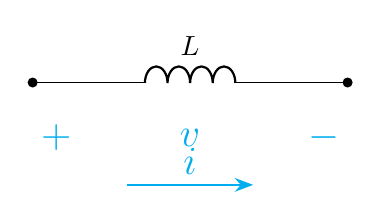
\begin{tikzpicture}
		% Draw the inductor with L label and filled nodes at ends
		\draw (0,0) to[L, l=$L$, *-*] (4,0);
		
		% Blue ink annotations for voltage v
		\node[cyan] at (0.3, -0.7) {\Large $+$};
		\node[cyan] at (3.7, -0.7) {\Large $-$};
		\node[cyan] at (2, -0.7) {\Large $v$};
		
		% Blue ink annotation for current i with an arrow
		\draw[-{Stealth}, cyan, thick] (1.2, -1.3) -- node[above] {\Large $i$} (2.8, -1.3);
	\end{tikzpicture}
	\end{center}
	$$i(t)=\frac{1}{L}\int^{t}_{t_{0}}v\;d\tau+i(t_{0})$$
	$$p=Li\frac{di}{dt}=\frac{dw}{dt}=vi(t)$$
	\subsubsection{Series}
	$$L_{eq}=\sum^{k}_{n=1}L_{n}$$
	\subsubsection{Parallel}
	$$L_{eq}=\frac{1}{\sum^{k}_{n=1}\frac{1}{L_{n}}}$$
	\subsection{Capacitor:}
	Made-up of two conductors seperated by an insulator. It acts as an O/C to DC current and S/C to AC. An important note to remember that electrical charge is not directly transported through the capacitor.
	\begin{center}
	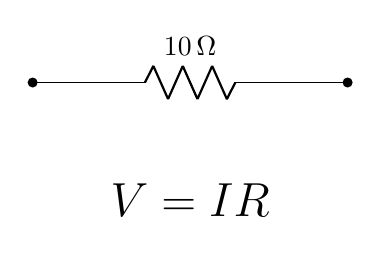
\begin{tikzpicture}
		% Resistor with 10 Ohm label
		\draw (0,0) to[R, l=$10\,\Omega$, *-*] (4,0);
		
		% V = IR equation below
		\node at (2, -1.5) {\LARGE $V = IR$};
	\end{tikzpicture}
	\end{center}
	$$i=C\frac{dv}{dt}$$
	$$v(t)=\frac{1}{C}\int^{t}_{t_{0}}i\;d\tau+v(t_{0})$$
	$$p=vi=Cv\frac{dv}{dt}$$
	$$w=\frac{1}{2}Cv^{2}$$
	\subsubsection{Series}
	$$C_{eq}=\frac{1}{\sum^{k}_{n=1}\frac{1}{C_{n}}}$$
	\subsubsection{Parallel}
	$$C_{eq}=\sum^{k}_{n=1}C_{n}$$
	\subsection{Mutual Inductance:}
	The magnetic fields between the two circuits create a mutual and self-\\-inductance voltages. Polarity of M depends on the way the coils are wound. $L_{1}$ and $L_{2}$ must be wound is opposing directions.
	\begin{center}
		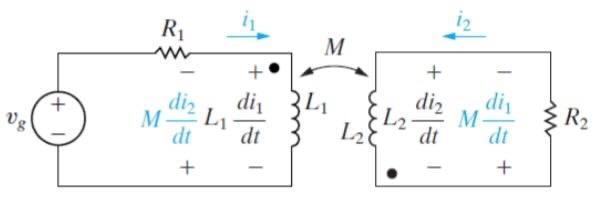
\includegraphics[scale=0.5]{mutual-inductance.png}
	\end{center}

	\section{Diodes}
	\subsection{Chemistry Revision:}
	Electrons form themselves into shells, with the outer shell containing the most energy due to their great mobility. These electrons in the outer shell are called valence electrons. Ions are formed through either an element donating or recieving electrons (e.g. Cations and Anions)
	\subsection{Energy Gaps:}
	Valence bonds within inter-elemental bonds are in the valence band. A conduction band is the energy band beyond the valence band.
	\begin{center}
		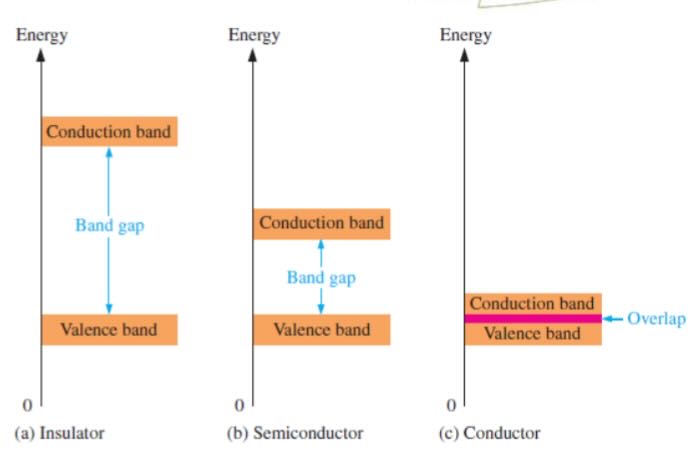
\includegraphics[scale=0.5]{energy-gaps.png}\\[1\baselineskip]
		\begin{tabular}{ | c | c |}
			\hline
			Material & $\rho(\Omega\cdot cm)$\\
			\hline
			Insulator & $\rho\;>\;10^{5}$\\
			Semiconductor & $10^{-5}\;<\rho\;<\;10^{5}$\\
			Conductor & $\rho\;<\;10^{-5}$\\
			\hline
		\end{tabular}
	\end{center}
	\subsection{Electrons and Holes:}
	\begin{center}
		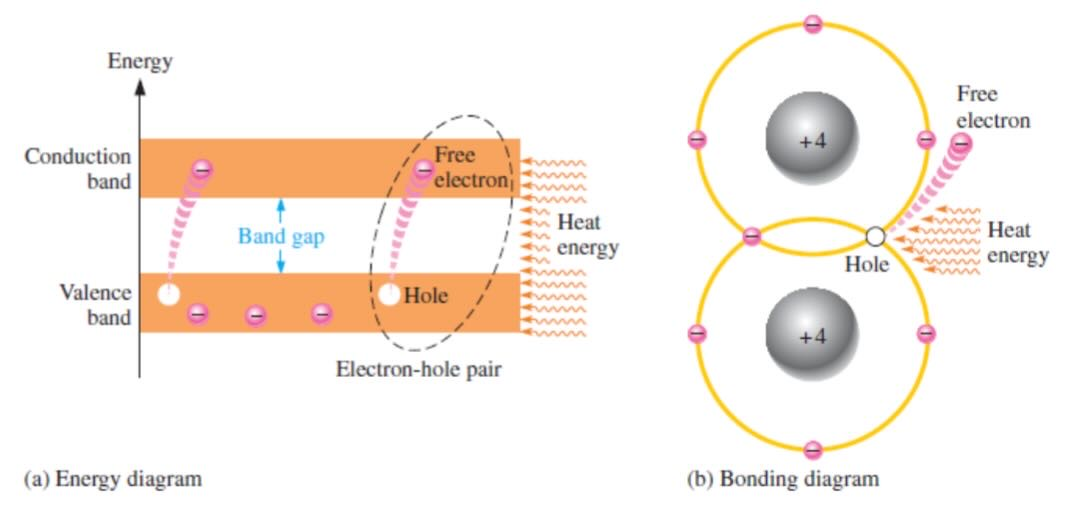
\includegraphics[scale=0.25]{electron-holes.png}
	\end{center}
	In instrinsic silicon it's current is produced by the movement of free electrons toward the end. The effective movement of the hole is opposite direction of electron movement.
	\subsection{Silicon:}
	\subsubsection{Doping Silicon}
	\paragraph{Donor Atoms}
	These atoms are pentavalent imparity, with 5 electrons in the valence shell. They are doped into the silicon crystal structure that donates the extra electron. This then becomes a conduction electron. 
	\paragraph{Acceptor Atoms}
	Place a trivalent imparity into the silicon crystal structure. Creating a hole within the silicon molecule.
	\subsubsection{PN Junction}
	In the image below, the acceptor is the \textit{p}-region and donor is \textit{n}-region. Within the PN-junction, the \textit{p}-region is negatively charged, and the \textit{n}-region is slightly positively charge.
	\begin{center}
		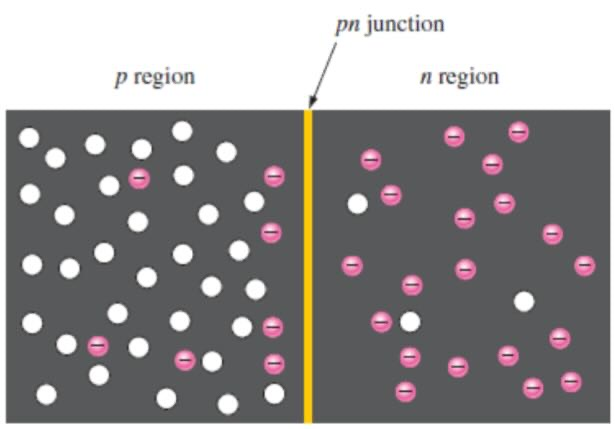
\includegraphics[scale=0.35]{pn-junction.png}
	\end{center}
	The PN-junction forms a basic diode. This is something that only allows current flow in one direction. A voltage drop is formed across the reigon as depletion of \textit{n}-type silicon and equillibrium occurs when it repel electron migration.
	\subsection{Diodes:}
	\subsubsection{Forward Bias}
	An external voltage assist electrons in moving through the PN-junction, allowing higher current flow. This reduces the width of the PN-junction.
	\begin{center}
		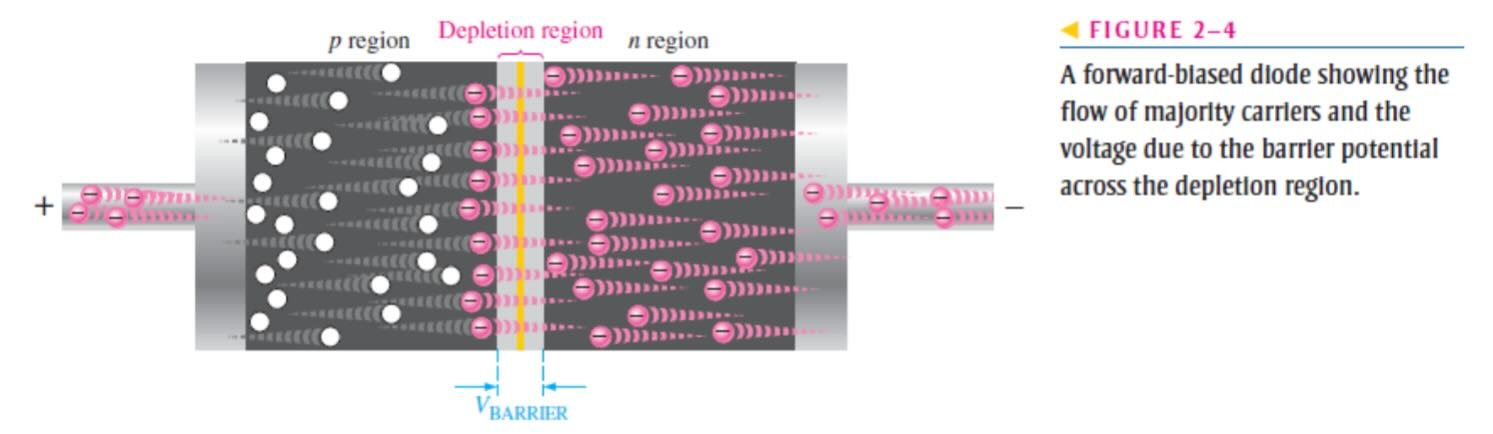
\includegraphics[scale=0.25]{diode-forward-bias.png}
	\end{center}
	\subsubsection{Reverse Bias}
	An extremely small reverse current pushes electrons back towards the PN-\\-junction.
	\begin{center}
		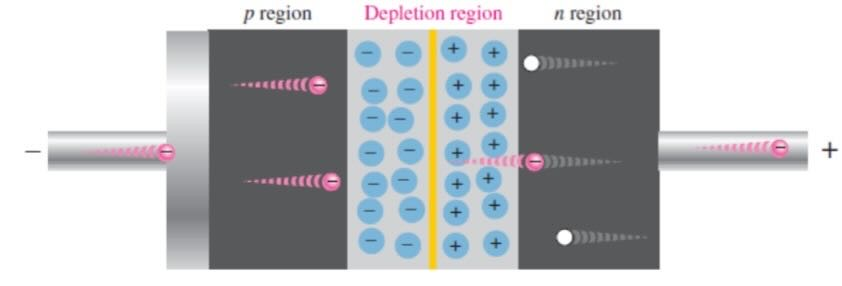
\includegraphics[scale=0.25]{diode-reverse-bais.png}
	\end{center}
	\subsection{Ideal Diode Models:}
	\subsubsection{Forward Bias}
	\begin{center}
	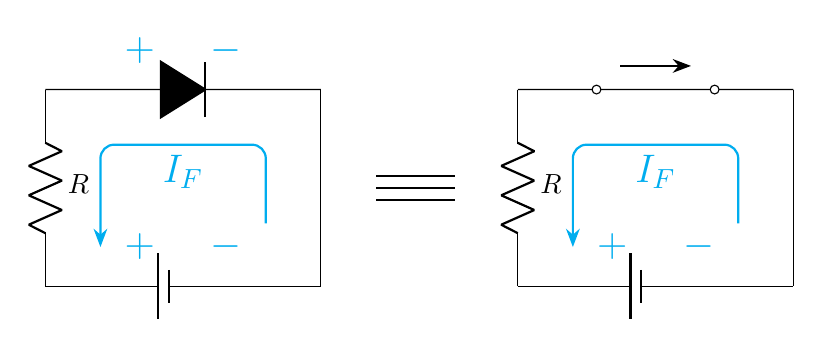
\begin{tikzpicture}
		% --- Left Circuit ---
		% Left branch with Resistor
		\draw (0,0) to[R, l_=$R$] (0,2.5);
		
		% Bottom branch with Battery
		\draw (0,0) -- (1,0) to[battery1] (2,0) -- (3.5,0);
		\node[cyan] at (1.2, 0.5) {\Large $+$};
		\node[cyan] at (2.3, 0.5) {\Large $-$};
		
		% Top branch with Diode (Filled)
		\draw (0,2.5) -- (1,2.5) to[D*] (2.5,2.5) -- (3.5,2.5);
		\node[cyan] at (1.2, 3) {\Large $+$};
		\node[cyan] at (2.3, 3) {\Large $-$};
		
		% Right branch
		\draw (3.5,2.5) to[short] (3.5,0);
		
		% Blue Loop for Current I_F
		\draw[-{Stealth}, cyan, thick, rounded corners=5pt] 
		    (2.8, 0.8) -- (2.8, 1.8) -- node[below] {\Large $I_F$} (0.7, 1.8) -- (0.7, 0.5);
		    
		    
		% --- Equivalence Symbol ---
		\draw[thick] (4.2, 1.4) -- (5.2, 1.4);
		\draw[thick] (4.2, 1.25) -- (5.2, 1.25);
		\draw[thick] (4.2, 1.1) -- (5.2, 1.1);


		% --- Right Circuit (Equivalent) ---
		\begin{scope}[shift={(6,0)}]
		    % Left branch with Resistor
		    \draw (0,0) to[R, l_=$R$] (0,2.5);
		    
		    % Bottom branch with Battery
		    \draw (0,0) -- (1,0) to[battery1] (2,0) -- (3.5,0);
		    \node[cyan] at (1.2, 0.5) {\Large $+$};
		    \node[cyan] at (2.3, 0.5) {\Large $-$};
		    
		    % Top branch with Closed Switch representation
		    \draw (0,2.5) -- (1,2.5) to[short, o-o] (2.5,2.5) -- (3.5,2.5);
		    % Arrow representing closed path current direction
		    \draw[-{Stealth}, thick] (1.3, 2.8) -- (2.2, 2.8);
		    
		    % Right branch
		    \draw (3.5,2.5) to[short] (3.5,0);
		    
		    % Blue Loop for Current I_F
		    \draw[-{Stealth}, cyan, thick, rounded corners=5pt] 
			(2.8, 0.8) -- (2.8, 1.8) -- node[below] {\Large $I_F$} (0.7, 1.8) -- (0.7, 0.5);
		\end{scope}
	\end{tikzpicture}
	\end{center}
	$$I_{F}=\frac{V_{BIAS}}{R_{LIMIT}}$$
	$$V_{F}=0V\text{, acts as S/C}$$
	\subsubsection{Reverse Bias}
	\begin{center}
	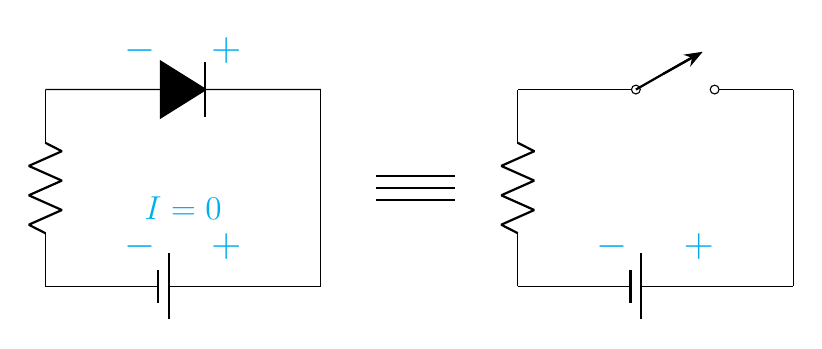
\begin{tikzpicture}
		% --- Left Circuit (Reverse Bias) ---
		% Left branch with Resistor
		\draw (0,0) to[R] (0,2.5);
		
		% Bottom branch with Battery
		% Drawing right-to-left so the short (negative) terminal is on the left
		\draw (0,0) -- (1,0);
		\draw (2,0) to[battery1] (1,0);
		\draw (2,0) -- (3.5,0);
		
		\node[cyan] at (1.2, 0.5) {\Large $-$};
		\node[cyan] at (2.3, 0.5) {\Large $+$};
		
		% Top branch with Diode
		\draw (0,2.5) -- (1,2.5) to[D*] (2.5,2.5) -- (3.5,2.5);
		\node[cyan] at (1.2, 3) {\Large $-$};
		\node[cyan] at (2.3, 3) {\Large $+$};
		
		% Right branch
		\draw (3.5,2.5) to[short] (3.5,0);
		
		% Center text I=0
		\node[cyan] at (1.75, 1) {\large $I=0$};
		    
		% --- Equivalence Symbol ---
		\draw[thick] (4.2, 1.4) -- (5.2, 1.4);
		\draw[thick] (4.2, 1.25) -- (5.2, 1.25);
		\draw[thick] (4.2, 1.1) -- (5.2, 1.1);

		% --- Right Circuit (Equivalent Open Circuit) ---
		\begin{scope}[shift={(6,0)}]
		    % Left branch with Resistor
		    \draw (0,0) to[R] (0,2.5);
		    
		    % Bottom branch with Battery (short terminal left)
		    \draw (0,0) -- (1,0);
		    \draw (2,0) to[battery1] (1,0);
		    \draw (2,0) -- (3.5,0);
		    
		    \node[cyan] at (1.2, 0.5) {\Large $-$};
		    \node[cyan] at (2.3, 0.5) {\Large $+$};
		    
		    % Top branch with Open Switch
		    \draw (0,2.5) -- (1.5,2.5) node[ocirc] {};
		    \draw[thick] (1.5,2.5) -- (2.2, 2.9);
		    \draw[-{Stealth}, thick] (1.85, 2.7) -- (2.35, 2.98);
		    \draw (2.5,2.5) node[ocirc] {} -- (3.5,2.5);
		    
		    % Right branch
		    \draw (3.5,2.5) to[short] (3.5,0);
		\end{scope}
	\end{tikzpicture}
	\end{center}
	$$I_{R}=0$$
	$$V_{R}=V_{BIAS}\text{, acts as O/C}$$
	\subsection{Practical Diode Models:}
	\subsubsection{Forward Bias}
	\begin{center}
	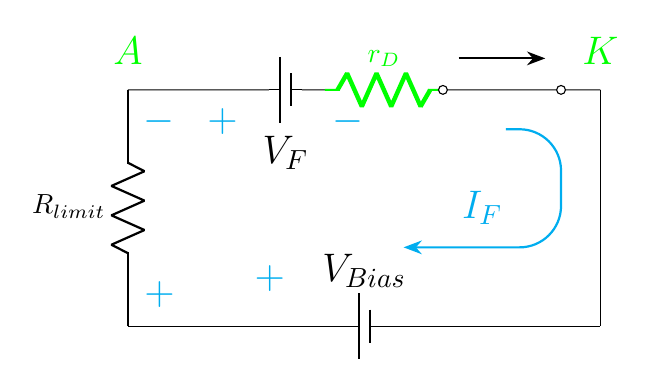
\begin{tikzpicture}
		% Nodes A and K (Green)
		\node[green, font=\Large] at (0, 3.5) {$A$};
		\node[green, font=\Large] at (6, 3.5) {$K$};
		
		% Left branch: R_limit
		\draw (0,0) to[R, l=$R_{limit}$] (0,3);
		% Blue signs for R_limit
		\node[cyan, font=\Large] at (0.4, 0.4) {$+$};
		\node[cyan, font=\Large] at (0.4, 2.6) {$-$};
		
		% Top branch: V_F, r_D (green), switch
		\draw (0,3) -- (1.5,3) to[battery1] (2.5,3);
		\node at (2, 2.2) {\Large $V_F$};
		\node[cyan, font=\Large] at (1.2, 2.6) {$+$};
		\node[cyan, font=\Large] at (2.8, 2.6) {$-$};
		
		% Dynamic resistance (Green)
		\draw[green, thick] (2.5,3) to[R, l=$r_D$] (4,3);
		
		% Closed Switch
		\draw (4,3) to[short, o-o] (5.5,3) -- (6,3);
		\draw[-{Stealth}, thick] (4.2, 3.4) -- (5.3, 3.4);
		
		% Right branch
		\draw (6,3) to[short] (6,0);
		
		% Bottom branch: V_Bias
		\draw (0,0) -- (2.5,0) to[battery1] (3.5,0) -- (6,0);
		\node at (3, 0.7) {\Large $V_{Bias}$};
		\node[cyan, font=\Large] at (1.8, 0.6) {$+$};
		
		% Blue Loop for I_F
		\draw[-{Stealth}, cyan, thick, rounded corners=15pt] 
		    (4.8, 2.5) -- (5.5, 2.5) -- (5.5, 1) -- (3.5, 1);
		\node[cyan, font=\Large] at (4.5, 1.5) {$I_F$};
		
	\end{tikzpicture}
	\end{center}
	$$V_{F}=0.7+I_{F}r'_{d}$$
	$$I_{F}=\frac{V_{BIAS}-0.7}{R_{LIMIT}+r'_{d}}$$
	\subsubsection{Reverse Bias}
	\begin{center}
	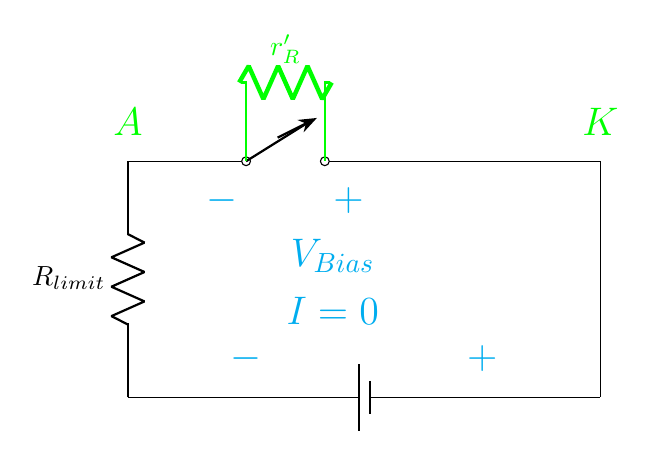
\begin{tikzpicture}
		% Nodes A and K (Green)
		\node[green, font=\Large] at (0, 3.5) {$A$};
		\node[green, font=\Large] at (6, 3.5) {$K$};
		
		% Left branch: R_limit
		\draw (0,0) to[R, l=$R_{limit}$] (0,3);
		
		% Top branch: Open Switch
		\draw (0,3) -- (1.5,3) node[ocirc] {};
		\draw[thick] (1.5,3) -- (2.3, 3.5);
		\draw[-{Stealth}, thick] (1.9, 3.3) -- (2.4, 3.55);
		\draw (2.5,3) node[ocirc] {} -- (6,3);
		
		% Reverse resistance r'_R across the switch (Green)
		\draw[green, thick] (1.5, 3) -- (1.5, 4) to[R, l=$r'_R$] (2.5, 4) -- (2.5, 3);
		
		% Voltage across switch markers
		\node[cyan, font=\Large] at (1.2, 2.5) {$-$};
		\node[cyan, font=\Large] at (2.8, 2.5) {$+$};
		
		% Center text
		\node[cyan, font=\Large] at (2.6, 1.8) {$V_{Bias}$};
		\node[cyan, font=\Large] at (2.6, 1.1) {$I=0$};
		
		% Right branch
		\draw (6,3) to[short] (6,0);
		
		% Bottom branch: V_Bias Battery
		\draw (0,0) -- (2.5,0) to[battery1] (3.5,0) -- (6,0);
		\node[cyan, font=\Large] at (1.5, 0.5) {$-$};
		\node[cyan, font=\Large] at (4.5, 0.5) {$+$};
	\end{tikzpicture}
	\end{center}
	The cathode side of the diode is connected to positive end of the power supply. Whereas, the anode is connected to the negative side.
	
	\section{Diode Applications}
	\subsection{Wave Rectifiers:}
	A rectifieris a type of circuit configurations that converts AC to its pulsating DC equivalent. A half-wave rectifier only converts half of the AC sine wave (e.g. positive or negative). A full wave rectifier converts the entirety of the sine wave.
	\begin{center}
	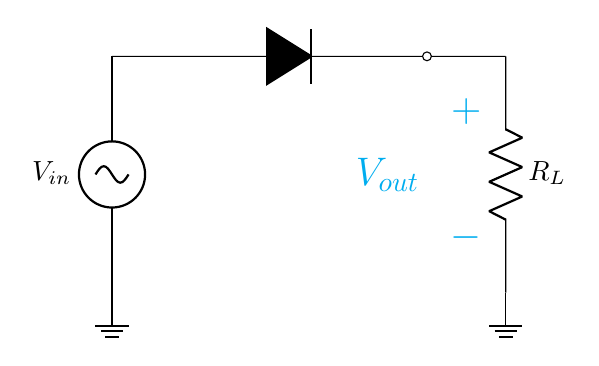
\begin{tikzpicture}
		% AC Voltage Source
		\draw (0,0) node[ground] {} 
			    to[sV, l=$V_{in}$] (0,3);
		
		% Top branch with Diode and test point
		\draw (0,3) -- (1,3) 
			    to[D*] (3.5,3) 
			    to[short, -o] (4,3) -- (5,3);
		
		% Load Resistor and Ground
		\draw (5,3) to[R, l=$R_L$] (5,0) 
			    node[ground] {};
		
		% Output Voltage Annotations
		\node[cyan, font=\Large] at (4.5, 2.3) {$+$};
		\node[cyan, font=\Large] at (4.5, 0.7) {$-$};
		\node[cyan, font=\Large] at (3.5, 1.5) {$V_{out}$};
	\end{tikzpicture}
	\end{center}
	For the circuit above, if $V_{in}$ is negative or smaller than the voltage barries in the diode, the diode should be reversed bias.
	\subsubsection{Half-wave operation}
	\begin{center}
		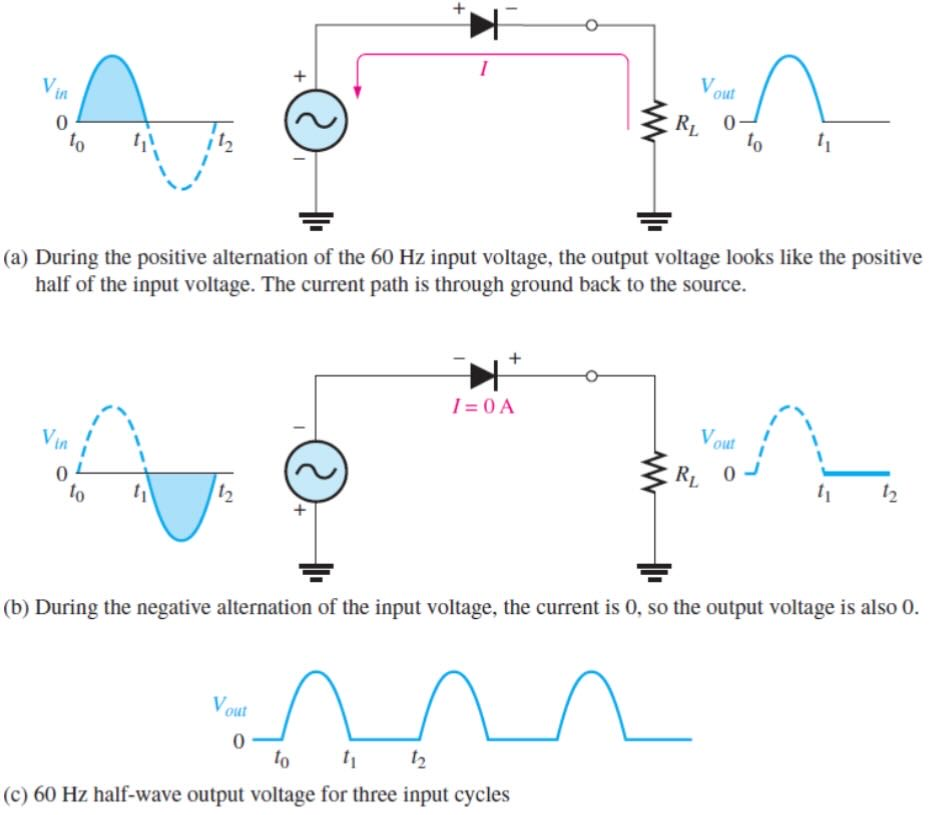
\includegraphics[scale=0.35]{half-wave-operation.png}
	\end{center}
	\subsubsection{Full-wave Rectifier}
	This circuit controls the direction of the load currents so that only the positive or negative outputs are recieved.
	\begin{center}
		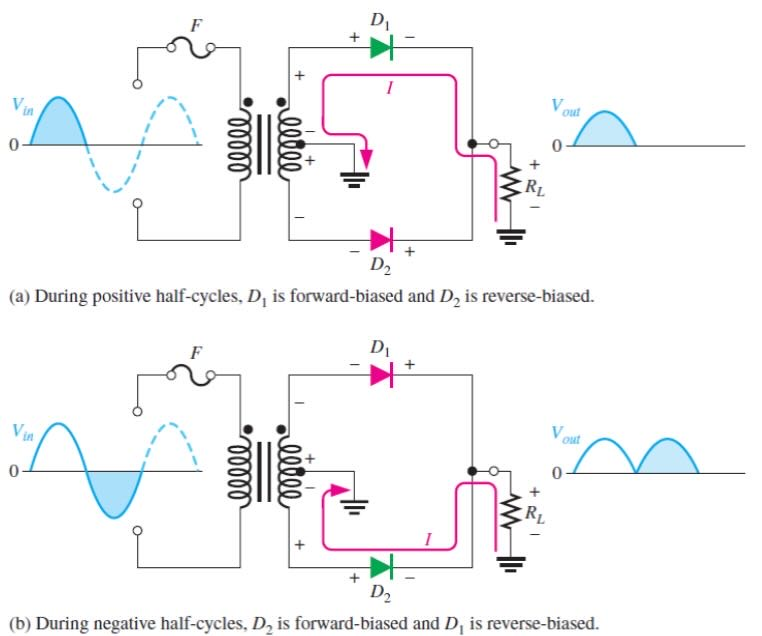
\includegraphics[scale=0.35]{full-wave-operation.png}
	\end{center}
	\subsubsection{Bridge Rectifier}
	\begin{center}
		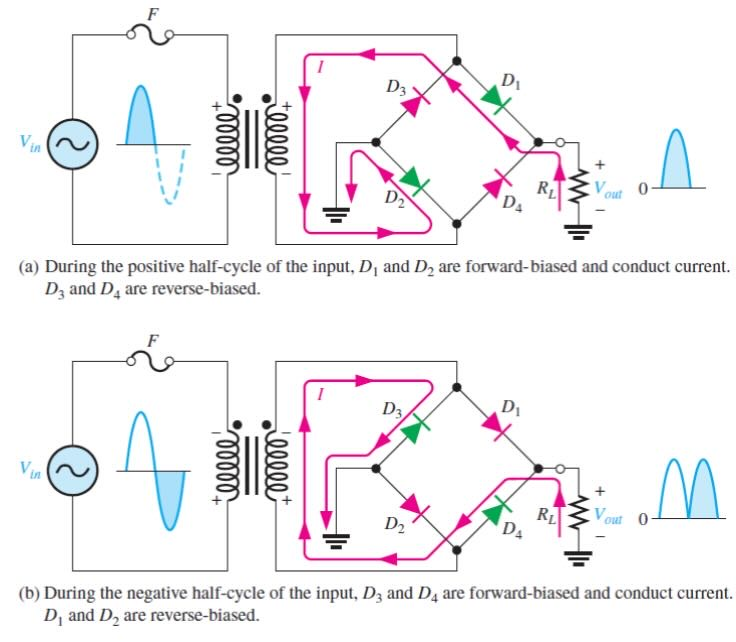
\includegraphics[scale=0.35]{bridge-rectifier.png}
	\end{center}
	\subsubsection{Smoothing Rectified Signal}
	The ripple within the output signal can put strain on connected DC comp\-onents. A capcitor is used to smooth the signal when the voltage no longer charges the capacitor. The larger the capacitor the small the ripple, and smoother the output voltage will be.
	\begin{center}
		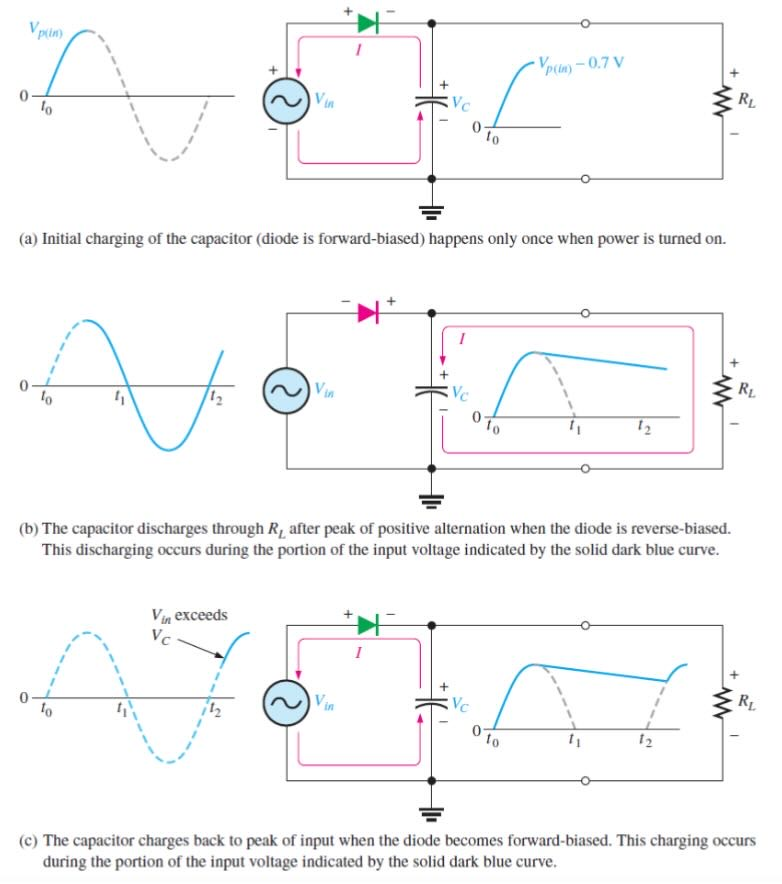
\includegraphics[scale=0.35]{rectification-smoothing.png}
	\end{center}
	\subsection{IC Regulators:}
	An intergrated circuit (IC) is a complete circuit on a small chip of silicon. The IC regulator is an IC connected to the output of a rectifier maintaining a consistent output voltage. The most common ones are 3-pin. The pins are for input, output, and reference adjustment.
	\subsection{Diode Limiters:}
	Limits the voltage to a certain value within the diode itself. The voltage is only limited to the circuit parallel to the diode. A common example of this is the Zener diode.
	\begin{center}
		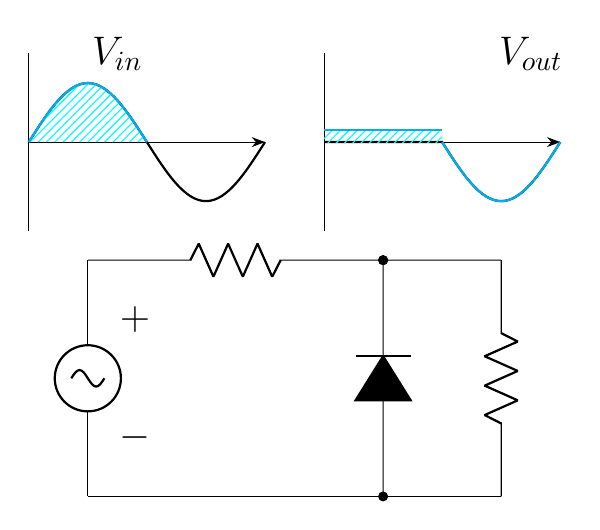
\begin{tikzpicture}[scale=0.75]
		% --- Top Left: Input Waveform (Vin) ---
		\begin{scope}[shift={(0, 6)}]
		    % Axes
		    \draw (0, -1.5) -- (0, 1.5);
		    \draw[-{Stealth}] (0, 0) -- (4, 0);
		    \node[font=\Large] at (1.5, 1.5) {$V_{in}$};
		    
		    % Sine wave
		    \draw[thick] (0,0) sin (1,1) cos (2,0) sin (3,-1) cos (4,0);
		    
		    % Cyan Shading for Positive Half-Cycle
		    \path[pattern=north east lines, pattern color=cyan] (0,0) sin (1,1) cos (2,0) -- cycle;
		    \draw[cyan, thick] (0,0) sin (1,1) cos (2,0);
		\end{scope}

		% --- Top Right: Output Waveform (Vout) ---
		\begin{scope}[shift={(5, 6)}]
		    % Axes
		    \draw (0, -1.5) -- (0, 1.5);
		    \draw[-{Stealth}] (0, 0) -- (4, 0);
		    \node[font=\Large] at (3.5, 1.5) {$V_{out}$};
		    
		    % Clipped wave
		    \draw[thick] (0,0) -- (2,0) sin (3,-1) cos (4,0);
		    
		    % Cyan Shading for Clipped Positive Half-Cycle
		    \path[pattern=north east lines, pattern color=cyan] (0,0) rectangle (2, 0.2);
		    \draw[cyan, thick] (0, 0.2) -- (2, 0.2);
		    \draw[cyan, thick] (2,0) sin (3,-1) cos (4,0);
		\end{scope}

		% --- Bottom: Circuit Diagram ---
		\begin{scope}[shift={(1, 0)}]
		    % AC Voltage Source
		    \draw (0,0) to[sV] (0,4);
		    \node[font=\Large] at (0.8, 3) {$+$};
		    \node[font=\Large] at (0.8, 1) {$-$};
		    
		    % Top branch with Series Resistor
		    \draw (0,4) -- (1,4) to[R] (4,4) to[short, -*] (5,4) -- (7,4);
		    
		    % Parallel Diode (Pointing Up)
		    \draw (5,0) to[D*, *-*] (5,4);
		    
		    % Load Resistor
		    \draw (7,4) to[R] (7,0);
		    
		    % Bottom Return Path
		    \draw (7,0) -- (0,0);
		\end{scope}
	\end{tikzpicture}
	\end{center}
	\subsection{Bias Limiters:}
	Similar to a diode limiter, but maintains a stable minimum voltage.
	\begin{center}
	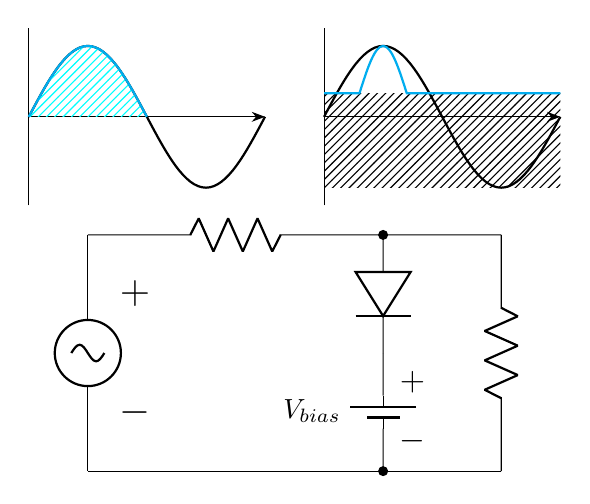
\begin{tikzpicture}[scale=0.75]
		% --- Top Left: Input Waveform ---
		\begin{scope}[shift={(0, 6)}]
		    % Axes
		    \draw (0, -1.5) -- (0, 1.5);
		    \draw[-{Stealth}] (0, 0) -- (4, 0);
		    
		    % Sine wave
		    \draw[thick] (0,0) sin (1,1.2) cos (2,0) sin (3,-1.2) cos (4,0);
		    
		    % Cyan Shading for Positive Half-Cycle
		    \path[pattern=north east lines, pattern color=cyan] (0,0) sin (1,1.2) cos (2,0) -- cycle;
		    \draw[cyan, thick] (0,0) sin (1,1.2) cos (2,0);
		\end{scope}

		% --- Top Right: Output Waveform ---
		\begin{scope}[shift={(5, 6)}]
		    % Axes
		    \draw (0, -1.5) -- (0, 1.5);
		    \draw[-{Stealth}] (0, 0) -- (4, 0);
		    
		    % Original unclipped wave (for reference)
		    \draw[thick] (0,0) sin (1,1.2) cos (2,0) sin (3,-1.2) cos (4,0);
		    
		    % Black shading representing the clipped portion
		    \path[pattern=north east lines, pattern color=black] (0,-1.2) rectangle (4, 0.4);
		    
		    % Cyan trace representing the clamped/minimum output voltage
		    \draw[cyan, thick] (0,0.4) -- (0.6,0.4) sin (1,1.2) cos (1.4,0.4) -- (4,0.4);
		\end{scope}

		% --- Bottom: Circuit Diagram ---
		\begin{scope}[shift={(1, 0)}]
		    % AC Voltage Source
		    \draw (0,0) to[sV] (0,4);
		    \node[font=\Large] at (0.8, 3) {$+$};
		    \node[font=\Large] at (0.8, 1) {$-$};
		    
		    % Top branch with Series Resistor
		    \draw (0,4) -- (1,4) 
				to[R] (4,4) 
				to[short, -*] (5,4) -- (7,4);
		    
		    % Parallel Branch: Diode and Bias Battery
		    \draw (5,4) to[D] (5,2);
		    \draw (5,2) to[battery1, l_=$V_{bias}$] (5,0);
		    \node[font=\large] at (5.5, 1.5) {$+$};
		    \node[font=\large] at (5.5, 0.5) {$-$};
		    
		    % Load Resistor
		    \draw (7,4) to[R] (7,0);
		    
		    % Bottom Return Path
		    \draw (7,0) -- (0,0);
		    \draw (5,0) to[short, *-] (5,0); % Connection dot
		\end{scope}
	\end{tikzpicture}
	\end{center}
	\subsection{Bias Variation:}
	\begin{center}
		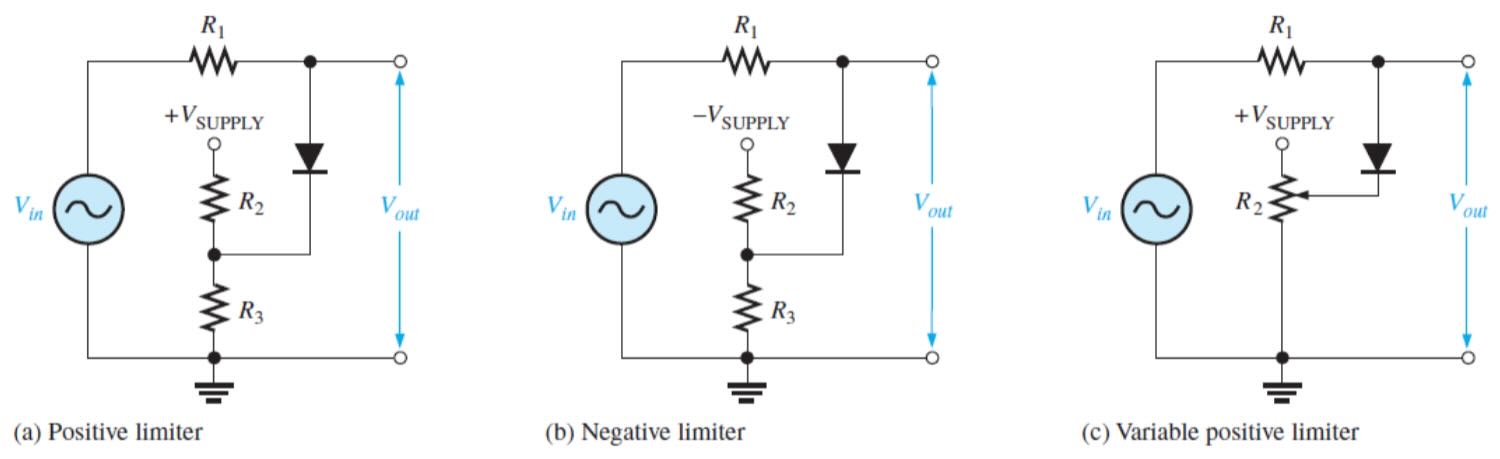
\includegraphics[scale=0.25]{bias-variation.png}
	\end{center}
	\subsection{Diode Clampers:}
	Adds a DC offset to an AC waveform. These can also be known as DC restorers.
	\begin{center}
		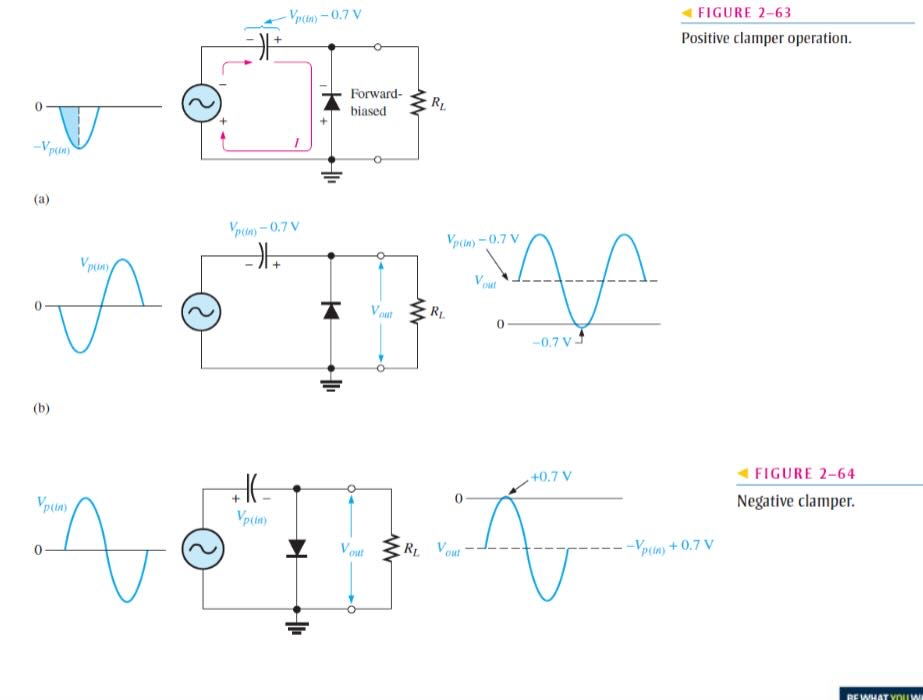
\includegraphics[scale=0.25]{diode-clampers.png}
	\end{center}
	\subsection{Extras:}
	PIV of a diode is just the complete negative of the input voltage. As the diode acts like a S/C. All diodes in series drop ~0.7V per diode.\\
	$V_{RMS}$ of half wave rectifier is:
	$$V_{RMS}=\frac{1}{\sqrt{2}}\cdot\frac{V_{out}}{2}$$
	$$V_{avg}=\frac{4V_{out}}{\pi}$$

	\section{Special Diodes}
	\subsection{Zener Diode:}
	A Zener diode is one which mainly operates in its reverse break-down region.
	\begin{center}
		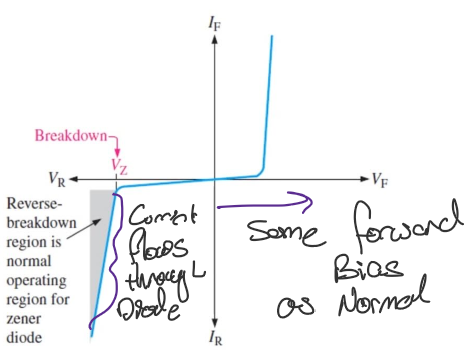
\includegraphics[scale=0.75]{zener-diode-CC.png}
	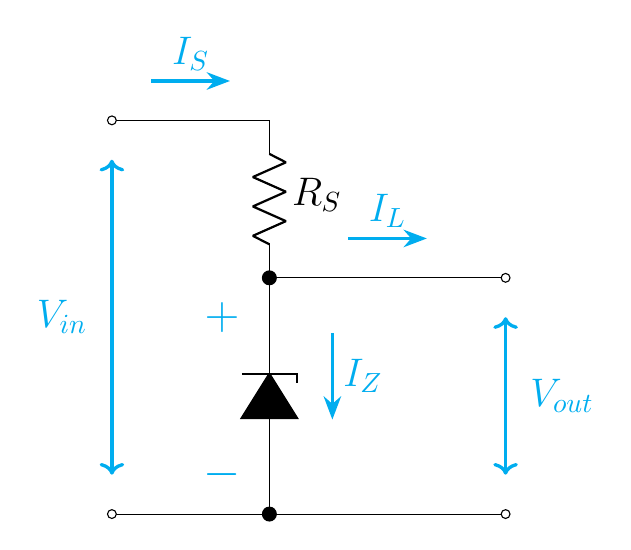
\begin{tikzpicture}[font=\Large]
		% --- Left side: Terminals and Input Voltage ---
		\draw (0,5) node[ocirc] {} -- (2,5);
		\draw (0,0) node[ocirc] {} -- (5,0);
		\draw[cyan, very thick, <->] (0, 0.5) -- (0, 4.5) node[midway, left=5pt] {$V_{in}$};

		% --- Top Branch: Series Resistor and Source Current ---
		% Source Current (Is) Arrow
		\draw[-{Stealth}, cyan, very thick] (0.5, 5.5) -- (1.5, 5.5) node[midway, above] {$I_S$};
		% Series Resistor (Rs)
		\draw (2,5) to[R, l=$R_S$] (2,3);

		% --- Middle Branch: Zener Diode ---
		% Filled Zener Diode (cathode up) using zD*
		\draw (2,3) to[zD*, invert] (2,0); 
		
		% Zener Current (Iz) Arrow and Voltage Polarity
		\draw[-{Stealth}, cyan, very thick] (2.8, 2.3) -- (2.8, 1.2) node[midway, right] {$I_Z$};
		\node[cyan, font=\LARGE] at (1.4, 2.5) {$+$};
		\node[cyan, font=\LARGE] at (1.4, 0.5) {$-$};

		% --- Right side: Output Branch and Load Current ---
		% Load Current (Il) Arrow
		\draw[-{Stealth}, cyan, very thick] (3, 3.5) -- (4, 3.5) node[midway, above] {$I_L$};
		% Terminals
		\draw (2,3) -- (5,3) node[ocirc] {};
		\draw (5,0) node[ocirc] {};
		
		% Output Voltage (Vout) Arrow
		\draw[cyan, very thick, <->] (5, 0.5) -- (5, 2.5) node[midway, right=5pt] {$V_{out}$};
		
		% --- Connection Dots ---
		\filldraw (2,3) circle (2.5pt);
		\filldraw (2,0) circle (2.5pt);
	\end{tikzpicture}
	\end{center}
	$$R_{S}=\frac{V_{in}-V_{out}}{I_{Z}}$$
	$$I_{Z(load)}=I_{Z(no load)}-I_{L}$$
	The breakdown voltage, is the ideal values for voltage items. After the maximum current through the diode. If more current is applied to the diode, permenant damage occurs. The knee current is the minimum current required for the voltage regulation to work properly.
	\subsection{Varactor Diode:}
	This diode is a reversed-biased PN-junction that utilizeds the inherent capacitence of the depletion region.
	\begin{center}
	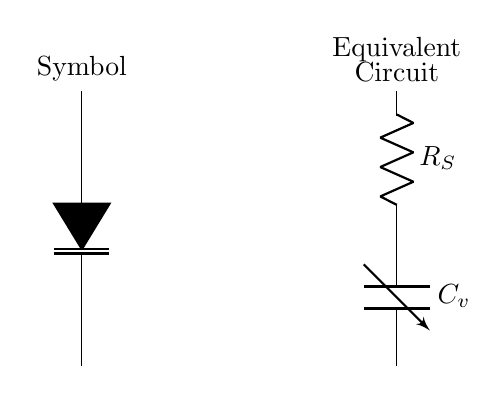
\begin{tikzpicture}
	    % --- Varactor Symbol ---
	    \node[above] at (0, 1) {Symbol};
	    \draw (0, 1) to[VC*] (0, -2.5);
	    
	    % --- Equivalent Circuit ---
	    \node[above, align=center] at (4, 1) {Equivalent\\[-0.3em]Circuit};
	    \draw (4, 1) to[american resistor, l=$R_S$] (4, -0.75)
			 to[variable capacitor, l=$C_v$] (4, -2.5);
	\end{tikzpicture}
	\end{center}
	\subsection{LightEmtting Diodes:}
	LEDsemit light when exposed to power. As such they are very useful as indicator throughoug a circuit. These diode types are designed to work only in forward bias conditions.
	\begin{center}
	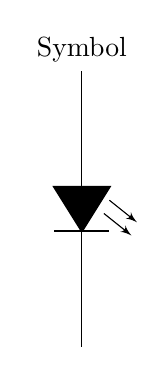
\begin{tikzpicture}
	    % --- LED Symbol ---
	    \node[above] at (0, 1) {Symbol};
	    \draw (0, 1) to [leD*] (0, -2.5);
	\end{tikzpicture}
	\end{center}
	\subsubsection{Organic LED:}
	The way OLED works is identical to the normal LEDS. The make-up of an OLED display is 2-3 layers, composed of organic polymers that emit light on certain voltage levels.
	\subsection{Photodiode:}
	A ligh absorbing device that conducts current based on light levels. This works in reverse bias configuration.
	\begin{center}
	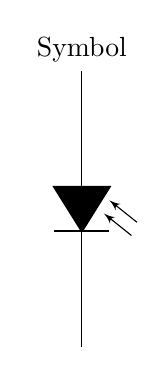
\begin{tikzpicture}
	    % --- Photodiode Symbol ---
	    \node[above] at (0, 1) {Symbol};
	    \draw (0, 1) to [pD*] (0, -2.5);
	\end{tikzpicture}
	\end{center}

	\section{Bipolar Junction Transistor}
	The following symbols are used to denote between the two types present. In where the types of silicon are placed within the silicon.
	\begin{center}
	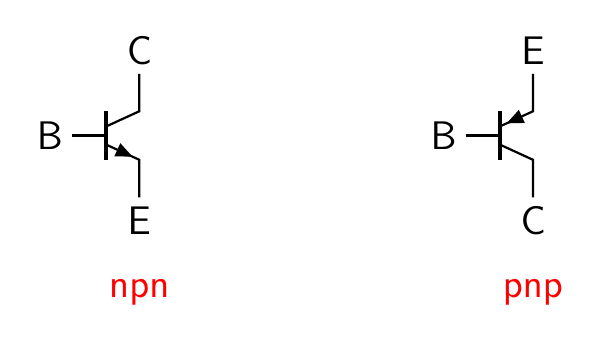
\begin{tikzpicture}[
	    thick,
	    font=\sffamily\Large,
	    term/.style={text=black, font=\sffamily\Large}
	]
			% --- NPN Transistor ---
	    % Using the standard npn node
	    \node[npn] (Q_npn) at (0, 0) {};
	    
	    % Terminal Labels
	    \node[term, left]  at (Q_npn.B) {B};
	    \node[term, above] at (Q_npn.C) {C};
	    \node[term, below] at (Q_npn.E) {E};
	    
	    % Type Label
	    \node[text=red] at (0, -2) {npn};

	    % --- PNP Transistor ---
	    % Using the standard pnp node, spaced 5 units to the right
	    \node[pnp] (Q_pnp) at (5, 0) {};
	    
	    % Terminal Labels
	    \node[term, left]  at (Q_pnp.B) {B};
	    \node[term, below] at (Q_pnp.C) {C};
	    \node[term, above] at (Q_pnp.E) {E};
	    
	    % Type Label
	    \node[text=red] at (5, -2) {pnp};

	\end{tikzpicture}
	\end{center}
	\subsection{BJT Biasing:}
	For a BJT to operate properly, it must be biased. The collector must be in reverse bias and emitter forward. The current direction opposes the direction the arrow is pointing.
	\begin{center}
		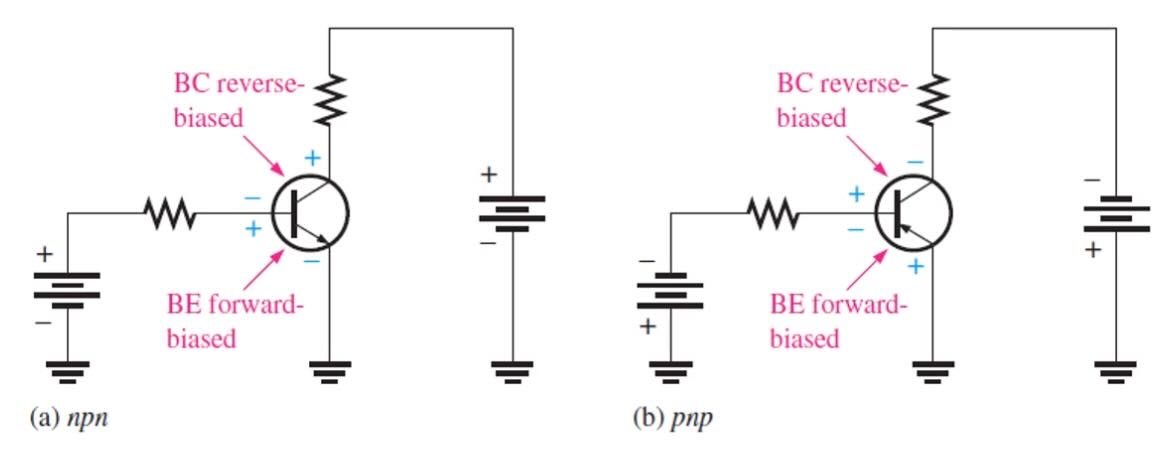
\includegraphics[scale=0.25]{bjt-biasing.png}
	\end{center}
	$$I_{E}=I_{B}+I_{C}$$
	Since base current is much lower than emittor or collector current the can equation equates to roughly $I_{E}\approx I_{C}$.
	\subsection{Beta DC:}
	$\beta_{DC}$ is the current gain of a transistor. On a datashett $\beta_{DC}$ is usually $h_{FE}$. This is only valid if the transistor operates within the manufacters specified range.
	$$\beta_{DC}=\frac{I_{C}}{I_{B}}$$
	$\beta_{DC}$ is not always a consistent value, as shown in the image below.
	\begin{center}
		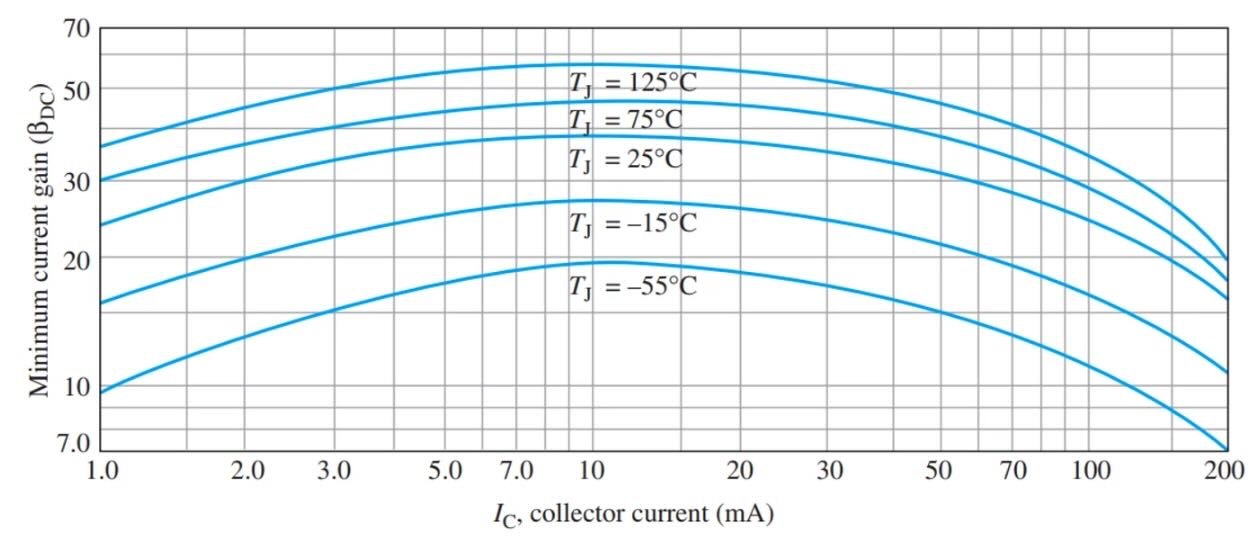
\includegraphics[scale=0.25]{beta-dc.png}
	\end{center}
	\subsection{Alpha DC:}
	$\alpha_{DC}$ is the ratio of the DC collector to DC emittor currents. Typical value ranges for $\alpha_{DC}$ is $0.95\rightarrow 0.99$. It is less common for $\alpha_{DC}$ to be found in the components datasheets than $\beta_{DC}$.
	\subsection{Equivalent Circuits:}
	\begin{center}
	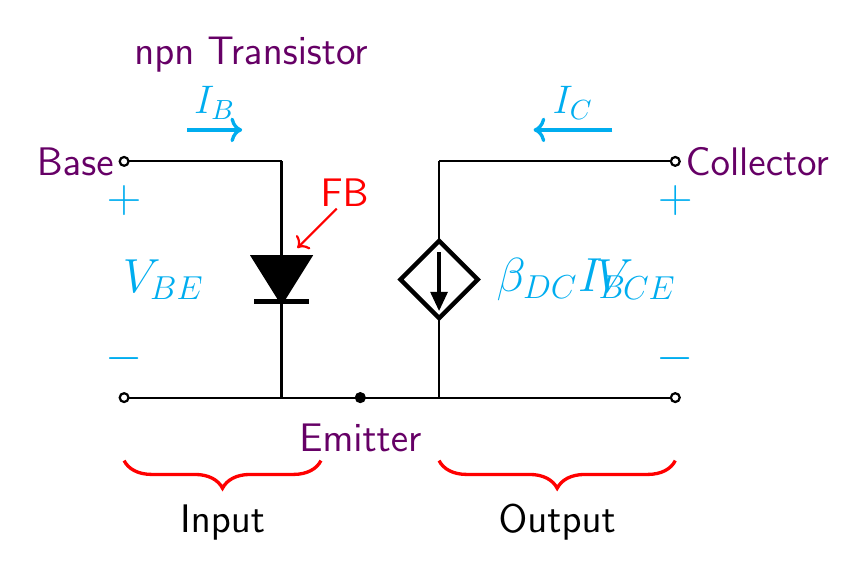
\begin{tikzpicture}[
	    thick,
	    font=\sffamily\Large,
	    cyan_label/.style={text=cyan, font=\LARGE},
	    purple_label/.style={text=violet!80!black},
	    red_label/.style={text=red}
	]

	    % --- Top Title ---
	    \node[purple_label, above right] at (0, 4) {npn Transistor};

	    % --- Left Side (Input) ---
	    % Base Terminal
	    \draw (0, 3) node[ocirc] {} node[purple_label, left] {Base}
		  -- (2, 3);
	    
	    % Input Voltage (V_BE)
	    \node[cyan_label] at (0.5, 1.5) {$V_{BE}$};
	    \node[cyan_label] at (0, 2.5) {$+$};
	    \node[cyan_label] at (0, 0.5) {$-$};

	    % Base Current (I_B)
	    \draw[->, cyan, very thick] (0.8, 3.4) -- (1.5, 3.4) node[midway, above] {$I_B$};

	    % Forward Biased Diode (Base to Emitter)
	    \draw (2, 3) to[D*] (2, 0);
	    \node[red_label] at (2.8, 2.6) {FB};
	    \draw[->, red, thick] (2.7, 2.4) -- (2.2, 1.9);

	    % Lower Input Terminal
	    \draw (0, 0) node[ocirc] {} -- (2, 0);

	    % --- Right Side (Output) ---
	    % Collector Terminal
	    \draw (7, 3) node[ocirc] {} node[purple_label, right] {Collector}
		  -- (4, 3);
		  
	    % Output Voltage (V_CE)
	    \node[cyan_label] at (6.5, 1.5) {$V_{CE}$};
	    \node[cyan_label] at (7, 2.5) {$+$};
	    \node[cyan_label] at (7, 0.5) {$-$};

	    % Collector Current (I_C)
	    % Corrected to point INWARDS (left) for an NPN model
	    \draw[->, cyan, very thick] (6.2, 3.4) -- (5.2, 3.4) node[midway, above] {$I_C$};

	    % Dependent Current Source
	    % Corrected to point DOWN (Collector to Emitter) for an NPN model
	    \draw (4, 3) to[cI] (4, 0);
	    \node[cyan_label, right] at (4.6, 1.5) {$\beta_{DC}I_B$};

	    % Lower Output Terminal
	    \draw (7, 0) node[ocirc] {} -- (4, 0);

	    % --- Common Emitter Line ---
	    \draw (2, 0) -- (4, 0);
	    \draw (3, 0) node[circ] {};
	    \node[purple_label, below=0.2cm] at (3, 0) {Emitter};

	    % --- Braces ---
	    \draw[decorate, decoration={brace, mirror, amplitude=10pt}, red, very thick] 
		(0, -0.8) -- (2.5, -0.8) node[midway, below=12pt, text=black] {Input};
		
	    \draw[decorate, decoration={brace, mirror, amplitude=10pt}, red, very thick] 
		(4, -0.8) -- (7, -0.8) node[midway, below=12pt, text=black] {Output};

	\end{tikzpicture}
	\end{center}
	\subsection{Voltage and Current:}
	\begin{center}
		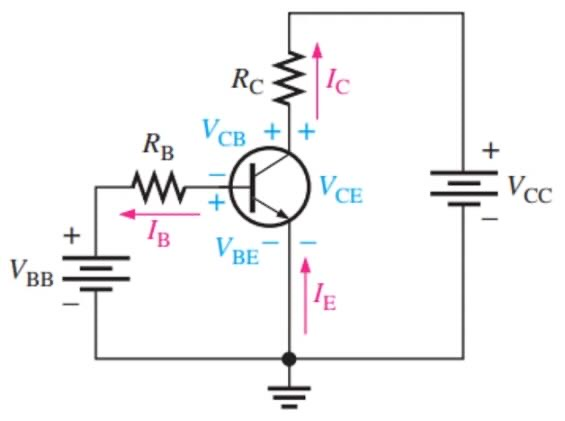
\includegraphics[scale=0.5]{bjt-current.png}
	\end{center}
	$$V_{BE}=0.7V$$
	$$I_{B}=\frac{V_{BB}-V_{BE}}{R_{B}}$$
	$$V_{CE}=V_{CC}-I_{C}R_{C}$$
	$$V_{CB}=V_{CE}-V_{BE}$$
	\subsection{Collector Characteristic Curves:}
	\begin{center}
		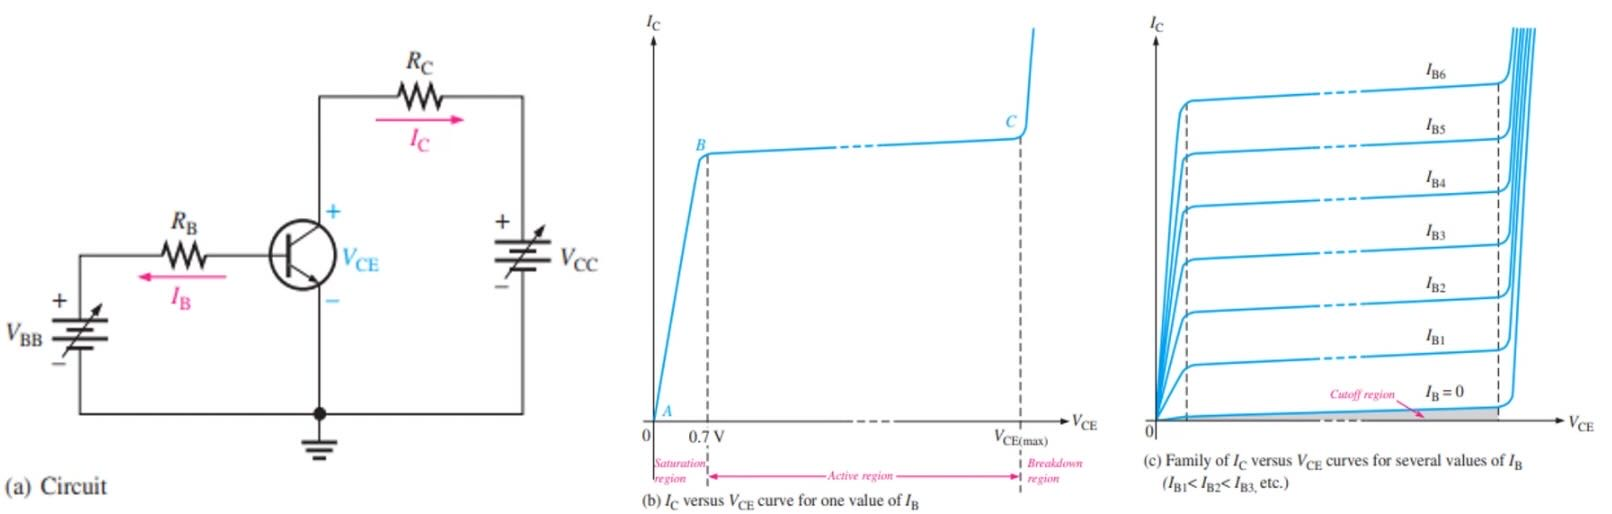
\includegraphics[scale=0.25]{bjt-cc.png}
	\end{center}
	\subsection{Cut-off:}
	When $I_{B}\approx 0$, the BJT is cut off and there is no collector current. In cut-off both base-emitter and base-collector are in reverse bias.
	\subsection{Saturation:}
	When base current is large, the $V_{CC}$ drop across $R_{C}$ is sufficient, leaving no voltage between the collector and emitter.
	$$I_{C(sat)}=\frac{V_{CC}}{R_{C}}$$
	$$I_{C(sat)}=\frac{V_{CC}-V_{CE(sat)}}{R_{C}}$$
	\subsection{Maximum Rating:}
	Transistors have limitations specified on the datasheet. As such the $V_{CE}$ and $I_{C}$ of the component must not exceed the $P_{D(max)}$. At higher temps the $P_{D(max)}$ is less.
	\subsection{BJT as an Amplifier:}
	$$V_{out}=\frac{R_{C}}{r'_{e}}\times V_{b}$$
	\begin{center}
		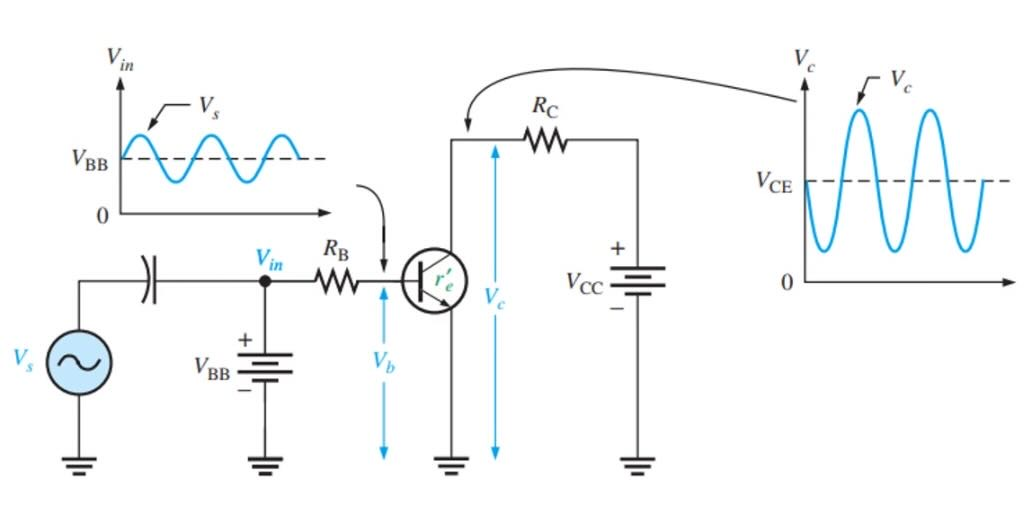
\includegraphics[scale=0.25]{bjt-amplifier.png}
	\end{center}
	\subsection{BJT as a Switch:}
	By switching a BJT in either cut-off or saturation, a basic switch can be formed. This is either through letting current not flow or flow through the transistor.
	\begin{center}
		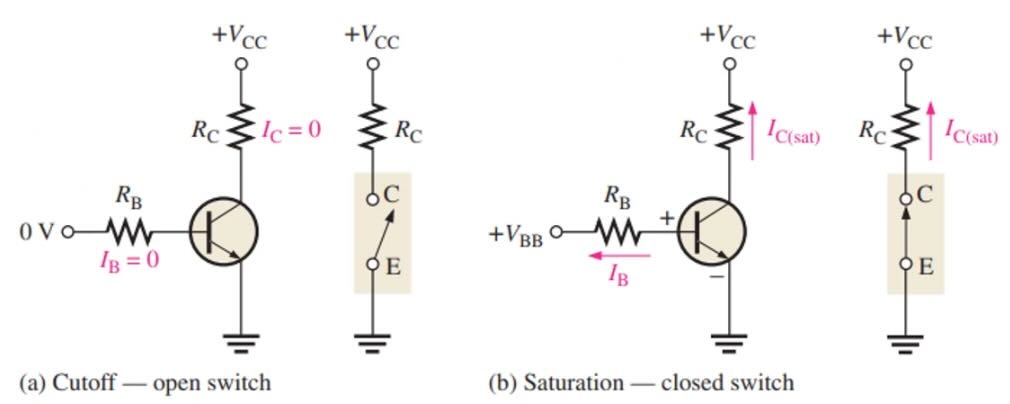
\includegraphics[scale=0.25]{bjt-switch.png}
	\end{center}

	\section{Transistor Bias Circuits}
	\subsection{Q Point - DC Operating Point:}
	The way a BJT amplifies a signal depends on it's biasing of itself.
	\subsection{Voltage Divider Biasing:}
	\begin{center}
		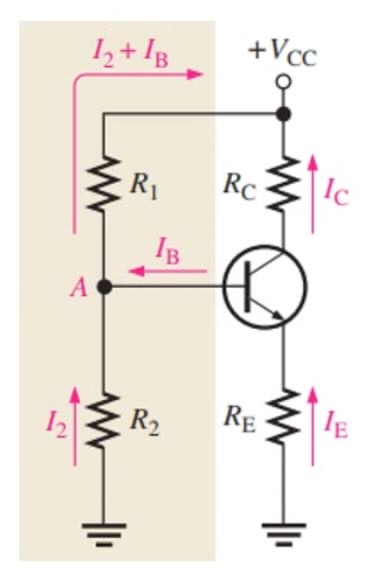
\includegraphics[scale=0.5]{bjt-voltage-divider-biasing.png}
	\end{center}
	\begin{align*}
		V_{B}&\approx\frac{R_{2}}{R_{1}+R_{2}}\times V_{CC}\\
		V_{BE}&=V_{B}-V_{E}\\
		      &\approx 0.7V\\
		I_{C}&\approx I_{E}\\
		     &=\frac{V_{E}}{R_{E}}\\
		V_{C}&=V_{CC}-I_{C}R_{C}\\
		V_{CE}&=V_{C}-V_{E}
	\end{align*}
	\subsection{DC Input Resistance:}
	Important as it is the resistance presented to an input signal coming into the base.
	\begin{align*}
		R_{in(Base)}&=\frac{V_{B}}{I_{B}}\\
			    &=\frac{\beta_{DC}V_{B}}{I_{E}}
	\end{align*}
	As it is the reliant upon $\beta_{DC}$, it will vary for different transistors at different temperatures.
	\subsection{Voltage Division with Thev\'evenin Equivalent Circuits:}
	\begin{center}
		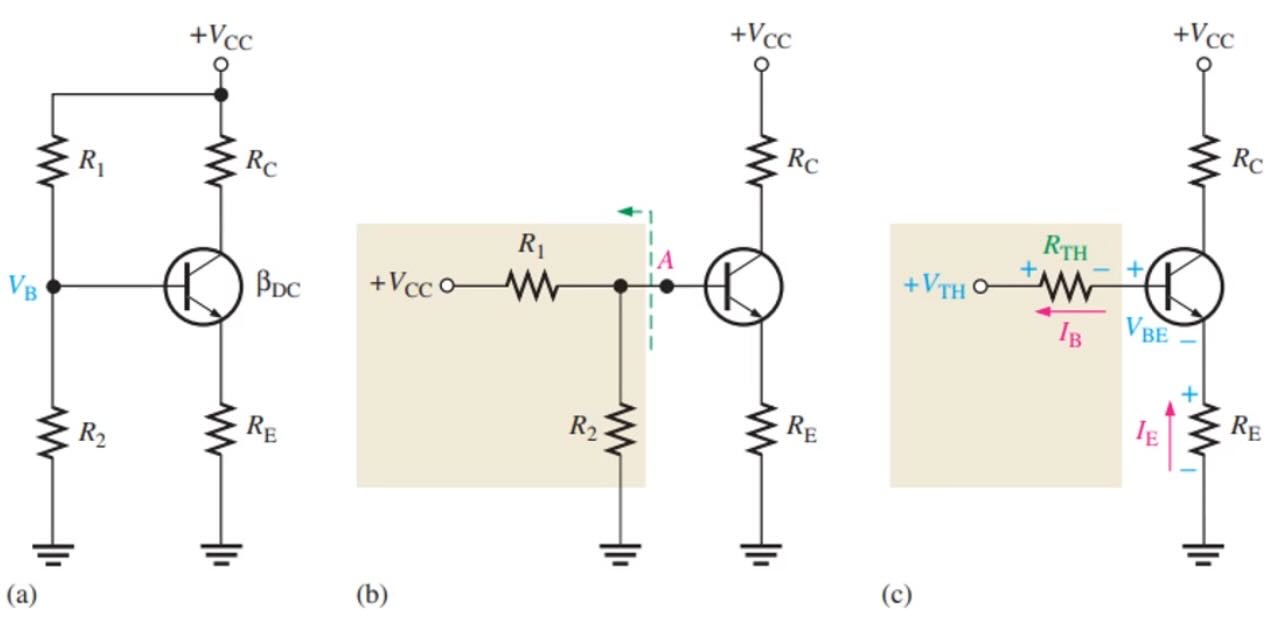
\includegraphics[scale=0.25]{voltage-divider-thevenin-equivalent.png}
	\end{center}
	$$V_{TH}=\frac{R_{2}}{R_{1}+R_{2}}V_{CC}$$
	$$R_{TH}=\frac{R_{1}R_{2}}{R_{1}+R_{2}}$$
	$$V_{TH}-V_{R_{TH}}-V_{BE}-V_{R_{E}}=0$$
	$$V_{TH}=F_{E}(R_{E}+\frac{R_{TH}}{\beta_{DC}})+V_{BE}$$
	$$F_{E}=\frac{V_{TH}-V_{BE}}{R_{E}+\frac{R_{TH}}{\beta_{DC}}}$$
	\subsection{Emitter Biasing:}
	\begin{center}
		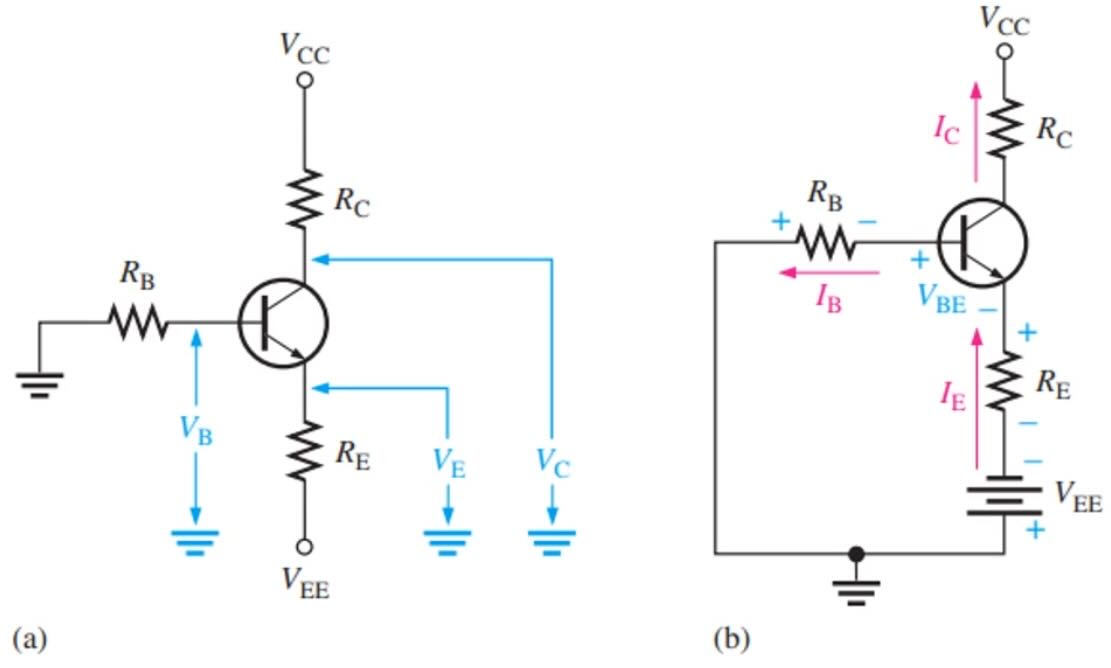
\includegraphics[scale=0.25]{emitter-biasing.png}
	\end{center}
	$$V_{EE}+V_{R_{B}}+V_{BE}+V_{R_{E}}=0$$
	\begin{align*}
		-V_{EE}&=\frac{I_{E}}{\beta_{DC}}R_{B}+I_{E}R_{E}+V_{BE}\\
		I_{E}&=\frac{-V_{EE}-V_{BE}}{R_{E}+\frac{R_{B}}{\beta_{DC}}}\\
		V_{E}&=V_{EE}+I_{E}R_{E}\\
		V_{B}&=V_{E}+V_{BE}\\
		V_{C}&=V_{CC}-I_{C}R_{C}
	\end{align*}
	\subsection{Base Biasing:}
	\begin{center}
		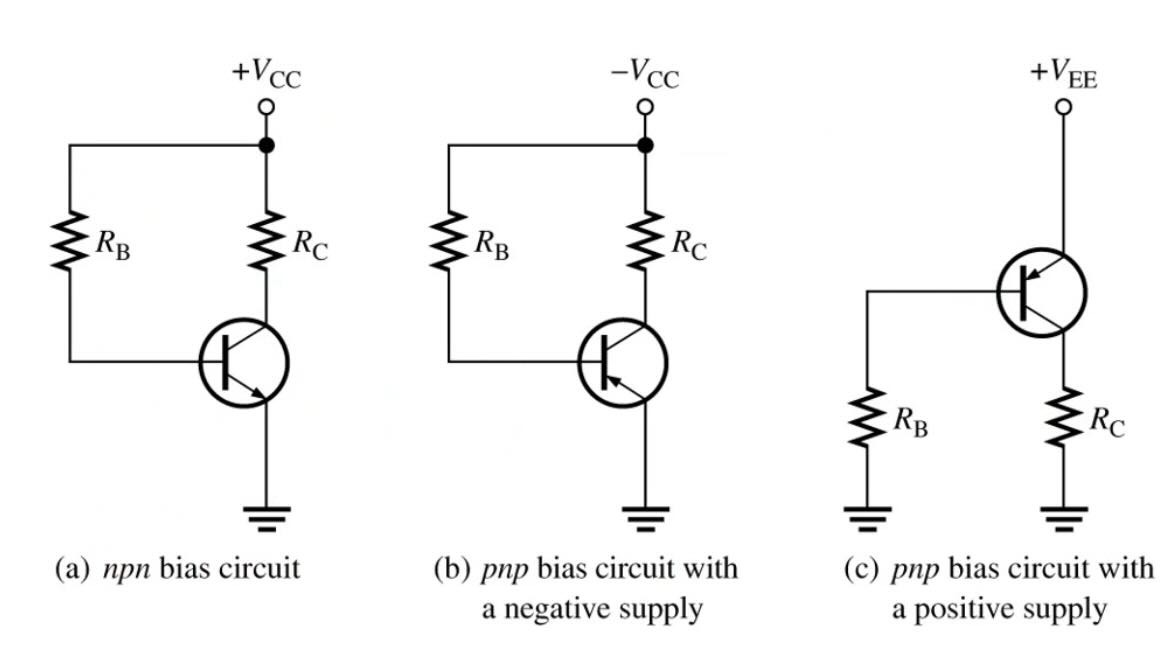
\includegraphics[scale=0.35]{base-biasing.png}
	\end{center}
	\begin{align*}
		V_{CC}-V_{R_{B}}-V_{BE}&=0\\
		V_{CC}-I_{B}R_{B}-V_{BE}&=0\\
		I_{B}&=\frac{V_{CC}-V_{BE}}{R_{B}}\\
		V_{CC}-I_{C}R_{C}-V_{CE}&=0\\
		V_{CE}&=V_{CC}-I_{C}R_{C}\\
		I_{C}&=\beta_{DC}(\frac{V_{CC}-V_{BE}}{R_{B}})
	\end{align*}
	\subsection{Emitter Feedback Biasing:}
	\begin{center}
		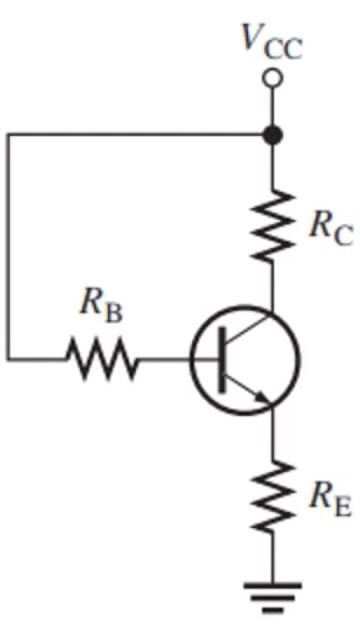
\includegraphics[scale=0.25]{emitter-feedback-biasing.png}
	\end{center}
	$$-V_{CC}+I_{B}R_{B}+V_{BE}+I_{E}R_{E}=0$$
	$$I_{E}=\frac{V_{CC}-V_{BE}}{R_{E}+\frac{R_{B}}{\beta_{DC}}}$$
	\subsection{Collector Feedback Biasing:}
	\begin{center}
		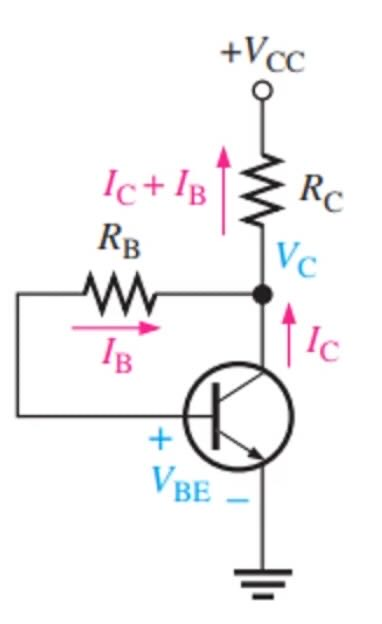
\includegraphics[scale=0.25]{collector-feedback-biasing.png}
	\end{center}
	\begin{align*}
		I_{B}&=\frac{V_{C}-V_{BE}}{R_{B}}\\
		     &=\frac{I_{C}}{\beta_{DC}}\\
		V_{C}&\approx V_{CC}-I_{C}R_{C}\\
		I_{C}&=\frac{V_{CC}-V_{BE}}{R_{C}+\frac{R_{B}}{\beta_{DC}}}\\
		V_{CE}&=V_{CC}-I_{C}R_{C}
	\end{align*}
	
	\section{Bipolar Junction Transistors as Amplifiers}
	\subsection{Tansistor AC Model:}
	\begin{center}
		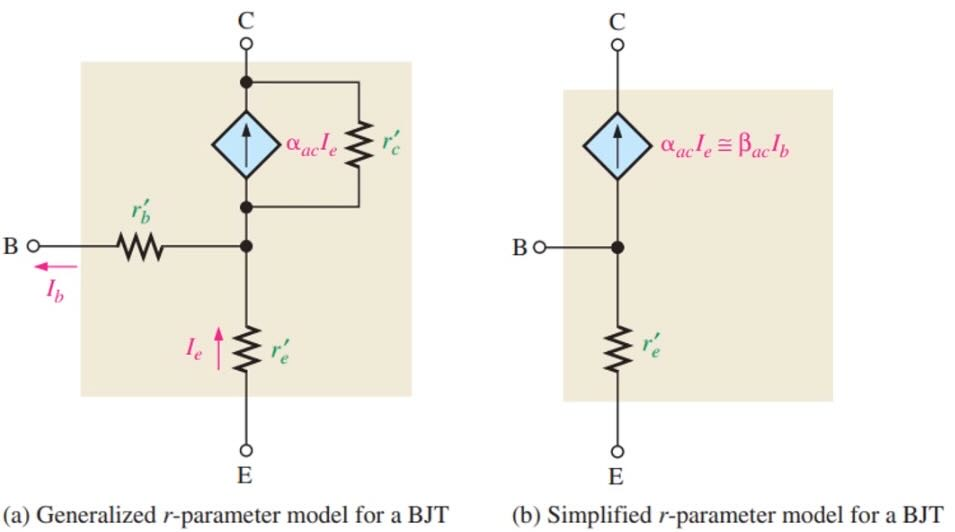
\includegraphics[scale=0.25]{bjt-ac.png}
		\begin{tabular}{ c | c }
			\hline
			Parameter & Description\\
			\hline
			$\alpha_{AC}$ & Alpha AC ($\frac{I_{C}}{I_{E}}$)\\
			$\beta_{AC}$ & Beta AC ($\frac{I_{C}}{I_{0}}$)\\
			$r'_{e}$ & AC Emitter Resistor\\
			$r'_{b}$ & AC Base Resistor\\
			$r'_{c}$ & AC Collector Resistor
		\end{tabular}
	\end{center}
	$$r'_{e}\approx\frac{25\text{mV}}{I_{E}}$$
	\subsection{Collector-Emitter Amplifier:}
	\begin{center}
		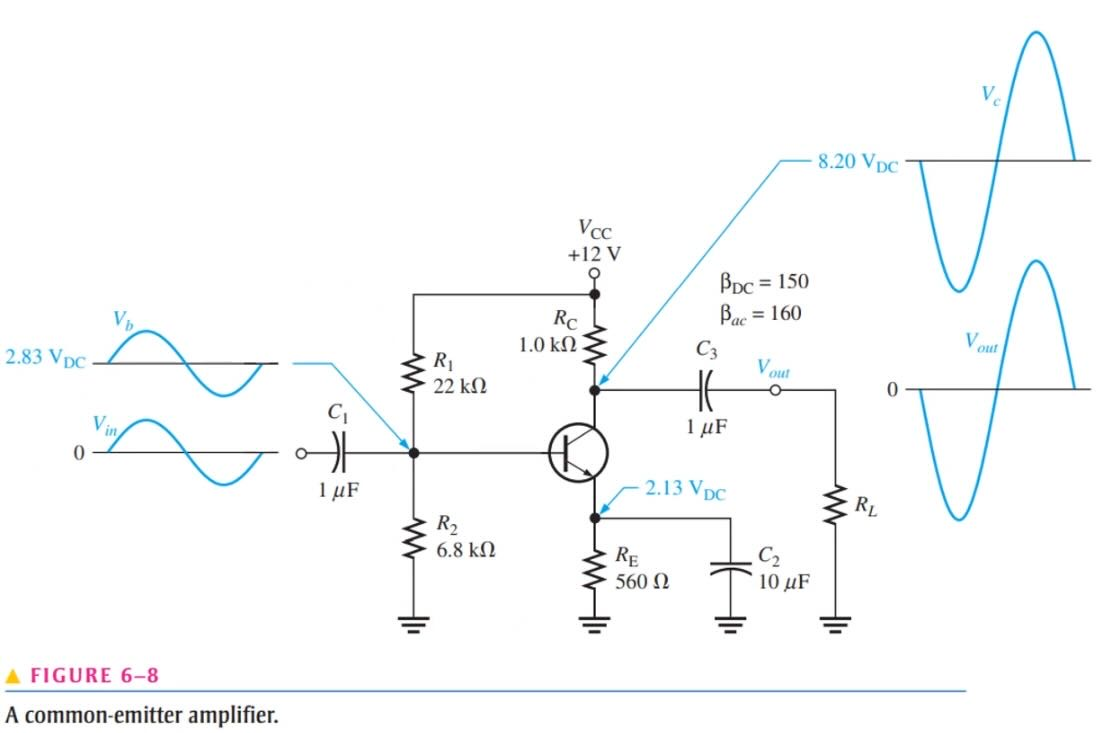
\includegraphics[scale=0.25]{ce-amplifier.png}
	\end{center}
	Useful for very high voltage and current gains. To calculate the CE amplifier, complete a DC analysis to find Q-point and $V_{CE}$. After, do the AC analysis.
	\begin{center}
		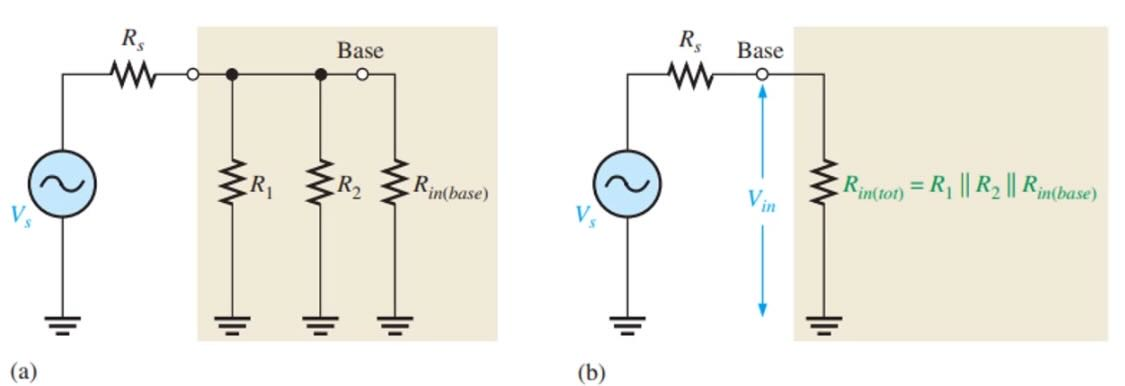
\includegraphics[scale=0.35]{ce-amplifier-base-resistance.png}
	\end{center}
	$$R_{in(tot)}=R_{1}||R_{2}||R_{in(base)}$$
	$$V_{b}=(\frac{R_{in(tot)}}{R_{s}+R_{in(tot)}})V_{s}$$
	\begin{center}
		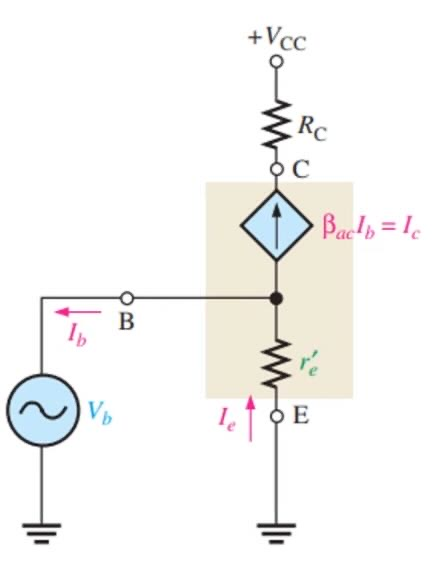
\includegraphics[scale=0.35]{ce-amplifier-ac-analysis.png}
	\end{center}
	\begin{align*}
		R_{in(base)}&=\frac{V_{in}}{I_{in}}\\
			    &=\frac{V_{b}}{I_{b}}\\
			    &=\frac{I_{e}r'_{e}}{I_{E}\/\beta_{ac}}\\
			    &=\beta_{ac}r'_{e}\\\\
		R_{out}&=R_{c}||r'_{e}\\
		       &=R_{C}||R_{L}
	\end{align*}
	\begin{center}
		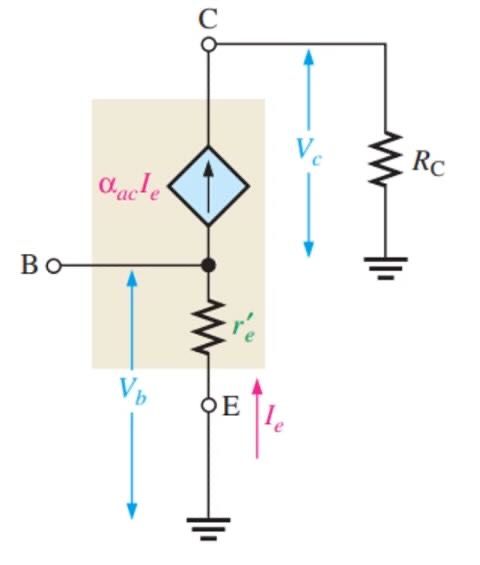
\includegraphics[scale=0.35]{ce-amplifier-amplification.png}
	\end{center}
	\begin{align*}
		V_{c}&=-\alpha_{ac}I_{E}R_{c}\\
		     &\approx-I_{E}R_{C}\\
		V_{b}&=I_{e}r'_{e}\\
		A_{V}=\frac{V_{c}}{V_{b}}\\
		     &=-\frac{R_{c}}{r'_{e}}
	\end{align*}
	The negative sign is used to indicate that the voltage is $180^{\circ}$ out of phase.
	\begin{align*}
		A_{i}&=\frac{I_{c}}{I_{s}}\\
		I_{s}&=\frac{V_{s}}{R_{s}+R_{in(tot)}}\\
		A_{P}&=A'_{v}A_{i}\\
		A'_{v}&=\frac{V_{c}}{V_{s}}
	\end{align*}
	\subsection{Emitter-follower Amplifier:}
	\begin{center}
		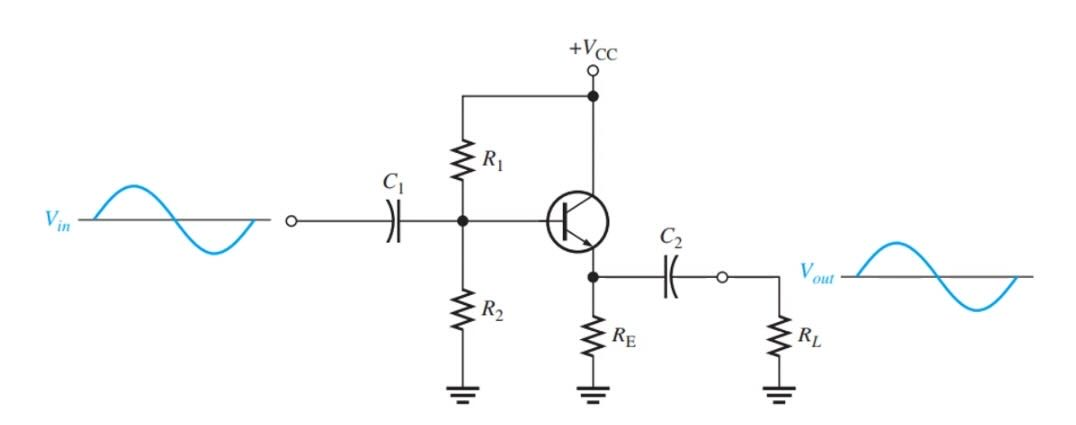
\includegraphics[scale=0.25]{cc-amplifier.png}
	\end{center}
	This type of amplifier is not great at voltage gain ($A_{v}\approx1$), but allows high current gain.
	$$V_{out}=I_{e}R_{e}$$
	$$V_{in}=I_{e}(r'_{e}+R_{e})$$
	$$A_{v}=\frac{R_{e}}{r'_{e}+R_{e}}$$
	When $V_{in}\approx V_{out}$, it has the same amplitude and phase-angle as the source.
	\begin{center}
		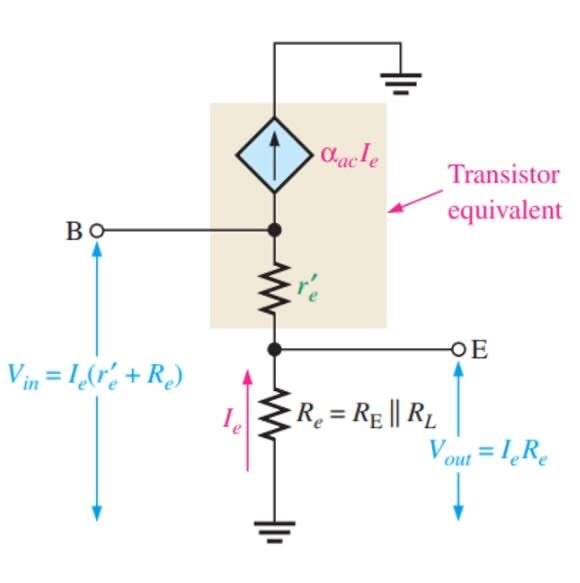
\includegraphics[scale=0.25]{ef-transistor-equivalent.png}
	\end{center}
	\begin{align*}
		A_{in(base)}&=\frac{V_{b}}{I_{b}}\\
			    &=\frac{I_{e}(r'_{e}+R_{e})}{I_{b}}\\
			    &=\beta_{ac}(r'_{e}+R_{eq})\\\\
		R_{in(tot)}&=R_{1}||R_{2}||R_{in(base)}\\
		R_{out}&\approx\frac{R_{s}}{\beta_{ac}}||R_{E}\\\\
		A_{i}&=\frac{I_{e}}{I_{in}}\\
		     &=\frac{I_{e}R_{in(tot)}}{V_{in}}\\
		A_{p}&=A_{v}A_{i}\\
		     &\approx A_{i},\text{ as $A_{v}\approx1$}
	\end{align*}
	\subsection{The Darlington Pair:}
	This is simply 2 cascading BJTs, with the emitter connected to the base of the other. The main advantage of using this is that it generates high input resistance and high current gain.
	\begin{center}
		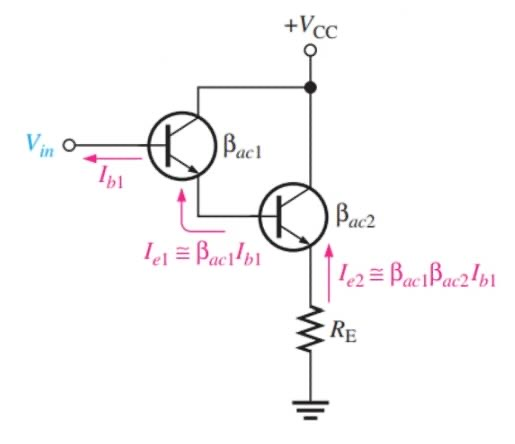
\includegraphics[scale=0.5]{darlington-pair.png}
	\end{center}
	$$\beta_{ac}=\beta_{ac1}\beta_{ac2}$$
	\subsection{Szikali Pair:}
	Use both npn and pnp BJTs. Its main advantage is low turn on voltage. With the most common application being used in conjuction with the Darlington pair.
	\begin{center}
		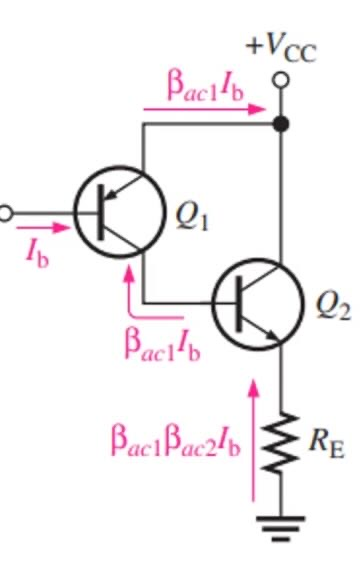
\includegraphics[scale=0.35]{szikali-pair.png}
	\end{center}
	\subsection{Collector-Base Amplifier:}
	\begin{center}
		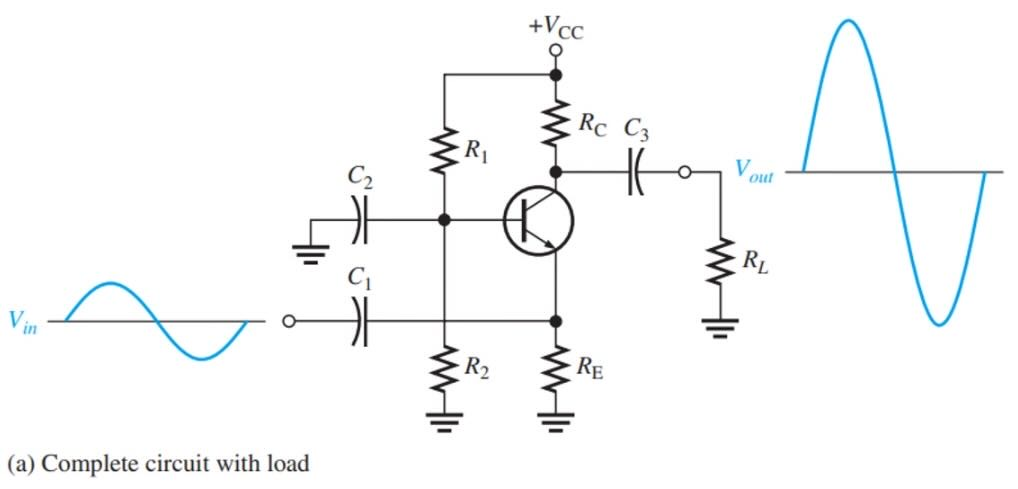
\includegraphics[scale=0.35]{cb-amplifier.png}
	\end{center}
	\begin{align*}
		A_{v}=&\frac{V_{c}}{V_{e}}\\
		=&\frac{I_{c}R_{c}}{I_{e}(r'_{e}||R_{e})}\\
		\approx&\frac{R_{c}||R_{L}}{r'_{e}}
	\end{align*}
	\begin{center}
		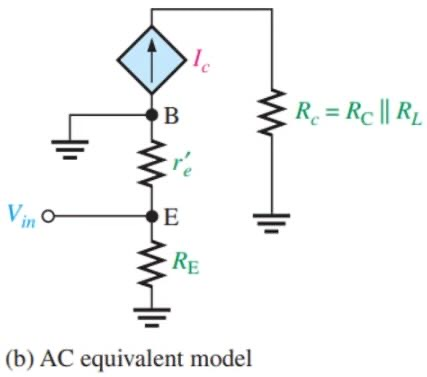
\includegraphics[scale=0.35]{cb-amplifier-ac.png}
	\end{center}
	\begin{align*}
		R_{in(emit)}=&\frac{V_{e}}{I_{e}}\\
		=&r'_{e}||R_{e}\\
		R_{out}\approx&R_{e}\\\\
		A_{v}=&\frac{r_{in}}{R_{L}}\\
		A_{i}=&1\\
		A_{p}\approx&A_{v}
	\end{align*}
\end{document}
